\documentclass[11pt,a4paper]{article}

\usepackage[utf8]{inputenc}
\usepackage[T1]{fontenc}
\usepackage{lmodern}
\usepackage[french]{babel}
\usepackage[margin=2.5cm]{geometry}
\usepackage{graphicx}
\usepackage{amsmath,amssymb}
\usepackage{booktabs}
\usepackage{array}
\usepackage{xcolor}
\usepackage[hidelinks]{hyperref}

\graphicspath{{figures/}{report/figures/}}
\setlength{\parskip}{0.5em}
\setlength{\parindent}{0pt}
\renewcommand{\arraystretch}{1.15}

\newcommand{\wine}{\textcolor[HTML]{8C2D4B}}

\title{\wine{\textbf{Classification de la qualité du vin}}\\[0.4em]\large Rapport technique -- Machine Learning 1}
\author{Kabore Boudnoma}
\date{Novembre 2026}

\begin{document}

\maketitle

\begin{abstract}
\noindent Ce rapport présente la construction d'un classifieur prédisant si un vin « Vinho Verde » est de bonne qualité
(note $\geq 7$) à partir de onze mesures physico-chimiques. Nous décrivons le prétraitement des données, la sélection de variables,
la comparaison de cinq familles de modèles du cours (régression logistique, $k$-NN, arbre de décision, Naive Bayes, SVM) complétés par des méthodes
d'ensemble, l'optimisation des hyperparamètres par Grid Search et Random Search, puis le choix d'un modèle final : un \emph{vote souple} de quatre modèles optimisés.
Ce modèle atteint sur le jeu de test un ROC-AUC de $0{,}864$ et un F1-score de $0{,}595$ pour la classe « bon vin ». Nous montrons que le plafond de
performance ($\approx 0{,}86$ d'AUC) provient de l'information contenue dans les variables plutôt que du choix de l'algorithme. Le code, les tests, une API
et une application web sont fournis.
\end{abstract}

\tableofcontents
\newpage

%% ------------------------------------------------------------------
\section{Introduction}

La qualité d'un vin dépend de nombreux paramètres physico-chimiques : acidité, pH, teneur en alcool, sucre résiduel, sulfites, etc.
L'objectif de ce projet est de développer un modèle de classification supervisée capable de prédire la qualité d'un vin à partir de ces
caractéristiques mesurables. Nous nous plaçons dans le cadre binaire demandé : un vin est jugé \emph{bon} si sa note est supérieure ou égale à 7.

\paragraph{Données.}
Nous utilisons les deux jeux de données publics de Cortez et al.~\cite{cortez2009} relatifs aux vins rouges (1\,599 échantillons) et blancs
(4\,898 échantillons) « Vinho Verde » du nord du Portugal, fusionnés en un seul jeu de $6\,497$ lignes. Chaque vin est décrit par onze variables continues
(acidité fixe, acidité volatile, acide citrique, sucre résiduel, chlorures, SO$_2$ libre, SO$_2$ total, densité, pH, sulfates, alcool) et par une
note de qualité entre 0 et 10, médiane d'au moins trois évaluations d'experts. Aucune information sur le cépage, la marque ou le prix n'est disponible.

\paragraph{Démarche.}
Le travail suit un protocole conçu pour éviter toute fuite d'information entre apprentissage et évaluation :
\begin{enumerate}
  \item analyse exploratoire et décisions de prétraitement (section~\ref{sec:data}) ;
  \item sélection de variables (section~\ref{sec:selection}) ;
  \item choix et justification des modèles (section~\ref{sec:modeles}) ;
  \item évaluation en validation croisée stratifiée à 5 plis sur le jeu d'entraînement (section~\ref{sec:eval}) ;
  \item optimisation des hyperparamètres (section~\ref{sec:tuning}) ;
  \item modèle final, seuil de décision et évaluation unique sur le jeu de test (section~\ref{sec:final}) ;
  \item mise en œuvre, tests et application (section~\ref{sec:impl}).
\end{enumerate}
Le jeu de test (20\,\% des données) n'est utilisé que pour l'évaluation finale. Toutes les opérations qui apprennent
des paramètres (standardisation, sélection de variables, seuil de décision) sont réalisées à l'intérieur de \texttt{Pipeline} scikit-learn~\cite{sklearn}
et réestimées dans chaque pli de validation croisée. La graine aléatoire est fixée (42).

%% ------------------------------------------------------------------
\section{Données et prétraitement}\label{sec:data}

\subsection{Statistiques descriptives}

Le tableau~\ref{tab:desc} résume les variables sur le jeu fusionné ($n = 6\,497$). Les onze variables sont numériques et continues, mais leurs échelles
diffèrent de plusieurs ordres de grandeur (de $\approx 0{,}01$ pour les chlorures à plus de $400$ pour le SO$_2$ total) : une standardisation sera nécessaire pour les
modèles sensibles aux distances ($k$-NN, SVM) et pour la régression logistique régularisée. Plusieurs variables sont fortement asymétriques à droite,
notamment les chlorures (asymétrie $5{,}4$), les sulfates ($1{,}8$), l'acidité fixe ($1{,}7$) et l'acidité volatile ($1{,}5$).

\begin{table}[htbp]
\centering\small
\caption{Statistiques descriptives du jeu fusionné (avant suppression des doublons).}\label{tab:desc}
\begin{tabular}{@{}lrrrrr@{}}
\toprule
Variable & Moyenne & Écart-type & Min & Max & Asymétrie \\
\midrule
Acidité fixe              & 7,215   & 1,296  & 3,80  & 15,90  & 1,72 \\
Acidité volatile          & 0,340   & 0,165  & 0,08  & 1,58   & 1,50 \\
Acide citrique            & 0,319   & 0,145  & 0,00  & 1,66   & 0,47 \\
Sucre résiduel            & 5,443   & 4,758  & 0,60  & 65,80  & 1,44 \\
Chlorures                 & 0,056   & 0,035  & 0,009 & 0,611  & 5,40 \\
SO$_2$ libre              & 30,53   & 17,75  & 1     & 289    & 1,22 \\
SO$_2$ total              & 115,75  & 56,52  & 6     & 440    & 0,00 \\
Densité                   & 0,995   & 0,003  & 0,987 & 1,039  & 0,50 \\
pH                        & 3,219   & 0,161  & 2,72  & 4,01   & 0,39 \\
Sulfates                  & 0,531   & 0,149  & 0,22  & 2,00   & 1,80 \\
Alcool                    & 10,492  & 1,193  & 8,0   & 14,9   & 0,57 \\
\midrule
Note (\texttt{quality})   & 5,818   & 0,873  & 3     & 9      & 0,19 \\
\bottomrule
\end{tabular}
\end{table}

\subsection{Valeurs manquantes et doublons}

Le jeu ne contient \textbf{aucune valeur manquante}. En revanche, $1\,177$ lignes (18,1\,\%) sont des doublons exacts (240 pour les rouges, 937 pour les blancs).
Nous avons vérifié qu'aucune combinaison de mesures identiques ne correspond à deux notes différentes. Conserver ces doublons provoquerait une
\textbf{fuite de données} : un même vin pourrait apparaître à la fois dans l'entraînement et dans le test, ce qui gonflerait artificiellement les scores. Ils sont donc
supprimés avant le découpage, ce qui laisse $5\,320$ vins.

\subsection{Variable cible et équilibre des classes}

La note est transformée en cible binaire \texttt{good} $= \mathbf{1}[\text{quality} \geq 7]$. Après suppression des doublons, la classe « bon vin » représente
\textbf{19\,\%} des observations (figure~\ref{fig:target}). Le problème est donc \emph{déséquilibré} (environ 81\,/\,19) : un classifieur qui prédit toujours « mauvais » obtient
81\,\% d'accuracy avec un rappel nul. L'accuracy seule est par conséquent trompeuse, et nous privilégions le F1-score de la classe positive, le rappel,
la précision, le ROC-AUC et l'AP (\emph{average precision}, aire sous la courbe précision-rappel). Les notes extrêmes sont très rares (5 vins à la note 9, 30 à la note 3),
ce qui rend une classification multiclasse peu fiable et justifie la binarisation. La proportion de bons vins diffère selon le type
(13,6\,\% pour les rouges, 21,6\,\% pour les blancs, avant suppression des doublons).

\begin{figure}[htbp]
\centering
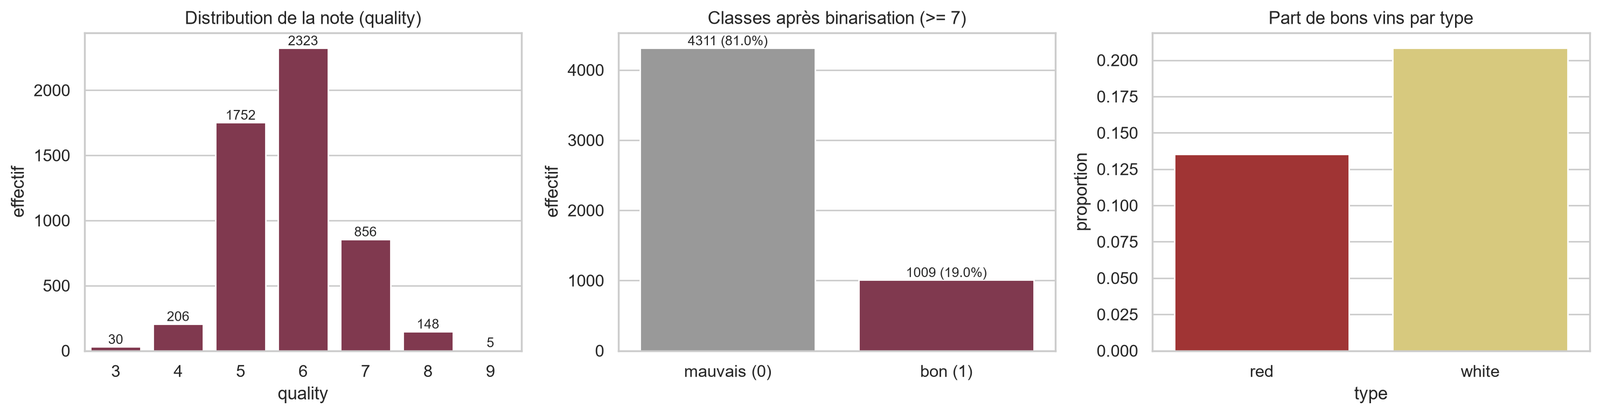
\includegraphics[width=\linewidth]{01_target_distribution.png}
\caption{Distribution de la note, équilibre des classes après binarisation et part de bons vins selon le type.}\label{fig:target}
\end{figure}

\subsection{Distributions et valeurs aberrantes}

Les histogrammes (figure~\ref{fig:hist}) confirment l'asymétrie de plusieurs variables. La règle de Tukey (1,5$\times$IQR) signale au moins une valeur aberrante
dans 20,6\,\% des lignes (8,1\,\% selon le critère $|z| > 3$), principalement pour l'acidité fixe, l'acidité volatile et les chlorures (figure~\ref{fig:box}).
Ces valeurs correspondent à des mesures physico-chimiques plausibles (vins très sucrés ou très salés) et non à des erreurs de saisie.
De plus, les lignes contenant une aberration comptent \emph{moins} de bons vins (12\,\% contre 21\,\%) : les supprimer appauvrirait encore la classe minoritaire.

\textbf{Décision} : les aberrations sont conservées. Nous les traitons par la robustesse : standardisation, transformation $\log(1+x)$ optionnelle des variables asymétriques
(comparée en validation croisée), et modèles peu sensibles (arbres, SVM à marge souple).

\begin{figure}[htbp]
\centering
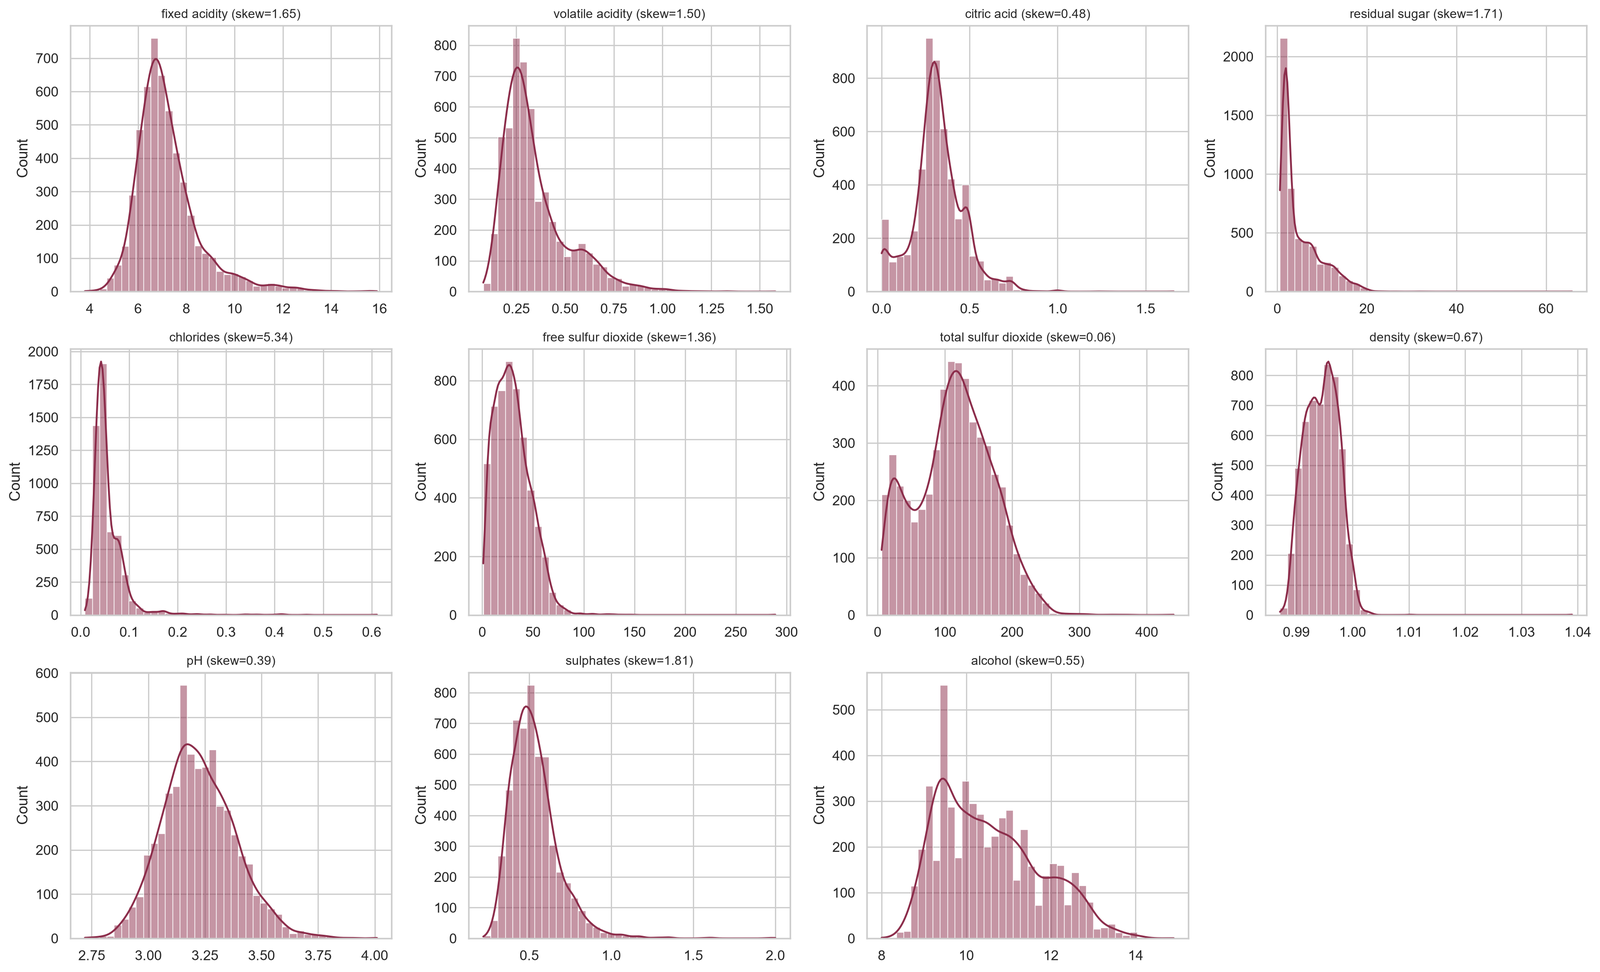
\includegraphics[width=\linewidth]{02_histograms.png}
\caption{Histogrammes des onze variables (jeu sans doublons) avec estimation de densité et asymétrie.}\label{fig:hist}
\end{figure}

\begin{figure}[htbp]
\centering
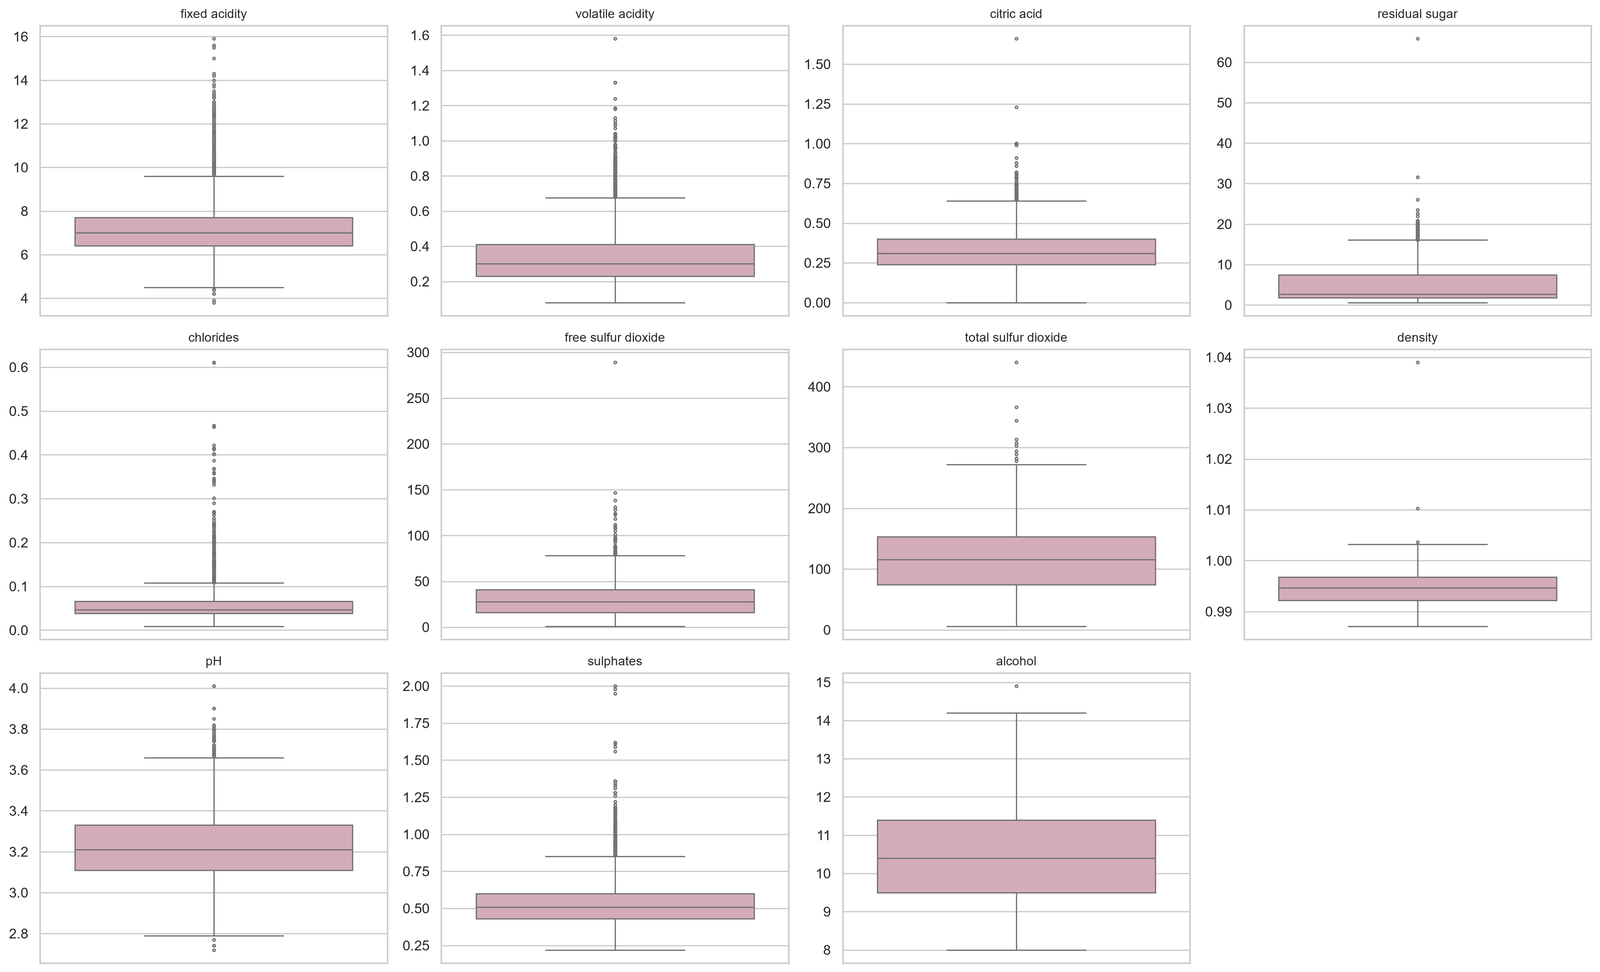
\includegraphics[width=\linewidth]{03_boxplots.png}
\caption{Boîtes à moustaches des onze variables.}\label{fig:box}
\end{figure}

\subsection{Corrélations et multicolinéarité}

La matrice de corrélation (figure~\ref{fig:corr}) révèle trois paires de variables corrélées à plus de 0,5 en valeur absolue :
SO$_2$ total et SO$_2$ libre ($r = 0{,}72$, le second étant inclus dans le premier), alcool et densité ($r = -0{,}67$) et densité et sucre résiduel ($r = 0{,}52$).
La densité est essentiellement déterminée par ces deux composantes. Pour quantifier la multicolinéarité nous calculons le facteur d'inflation de la variance
\begin{equation}
  \mathrm{VIF}_j = \frac{1}{1 - R_j^2},
\end{equation}
où $R_j^2$ est le coefficient de détermination de la régression de la variable $j$ sur les autres. Un VIF supérieur à 10 est généralement considéré comme problématique.
La densité atteint $14{,}9$, le sucre résiduel $6{,}4$, l'acidité fixe $4{,}9$ et l'alcool $4{,}6$ ; toutes les autres variables sont inférieures à $3$.
La multicolinéarité déstabilise les coefficients de la régression logistique ; elle justifie la régularisation et l'étude d'une sélection de variables.

\begin{figure}[htbp]
\centering
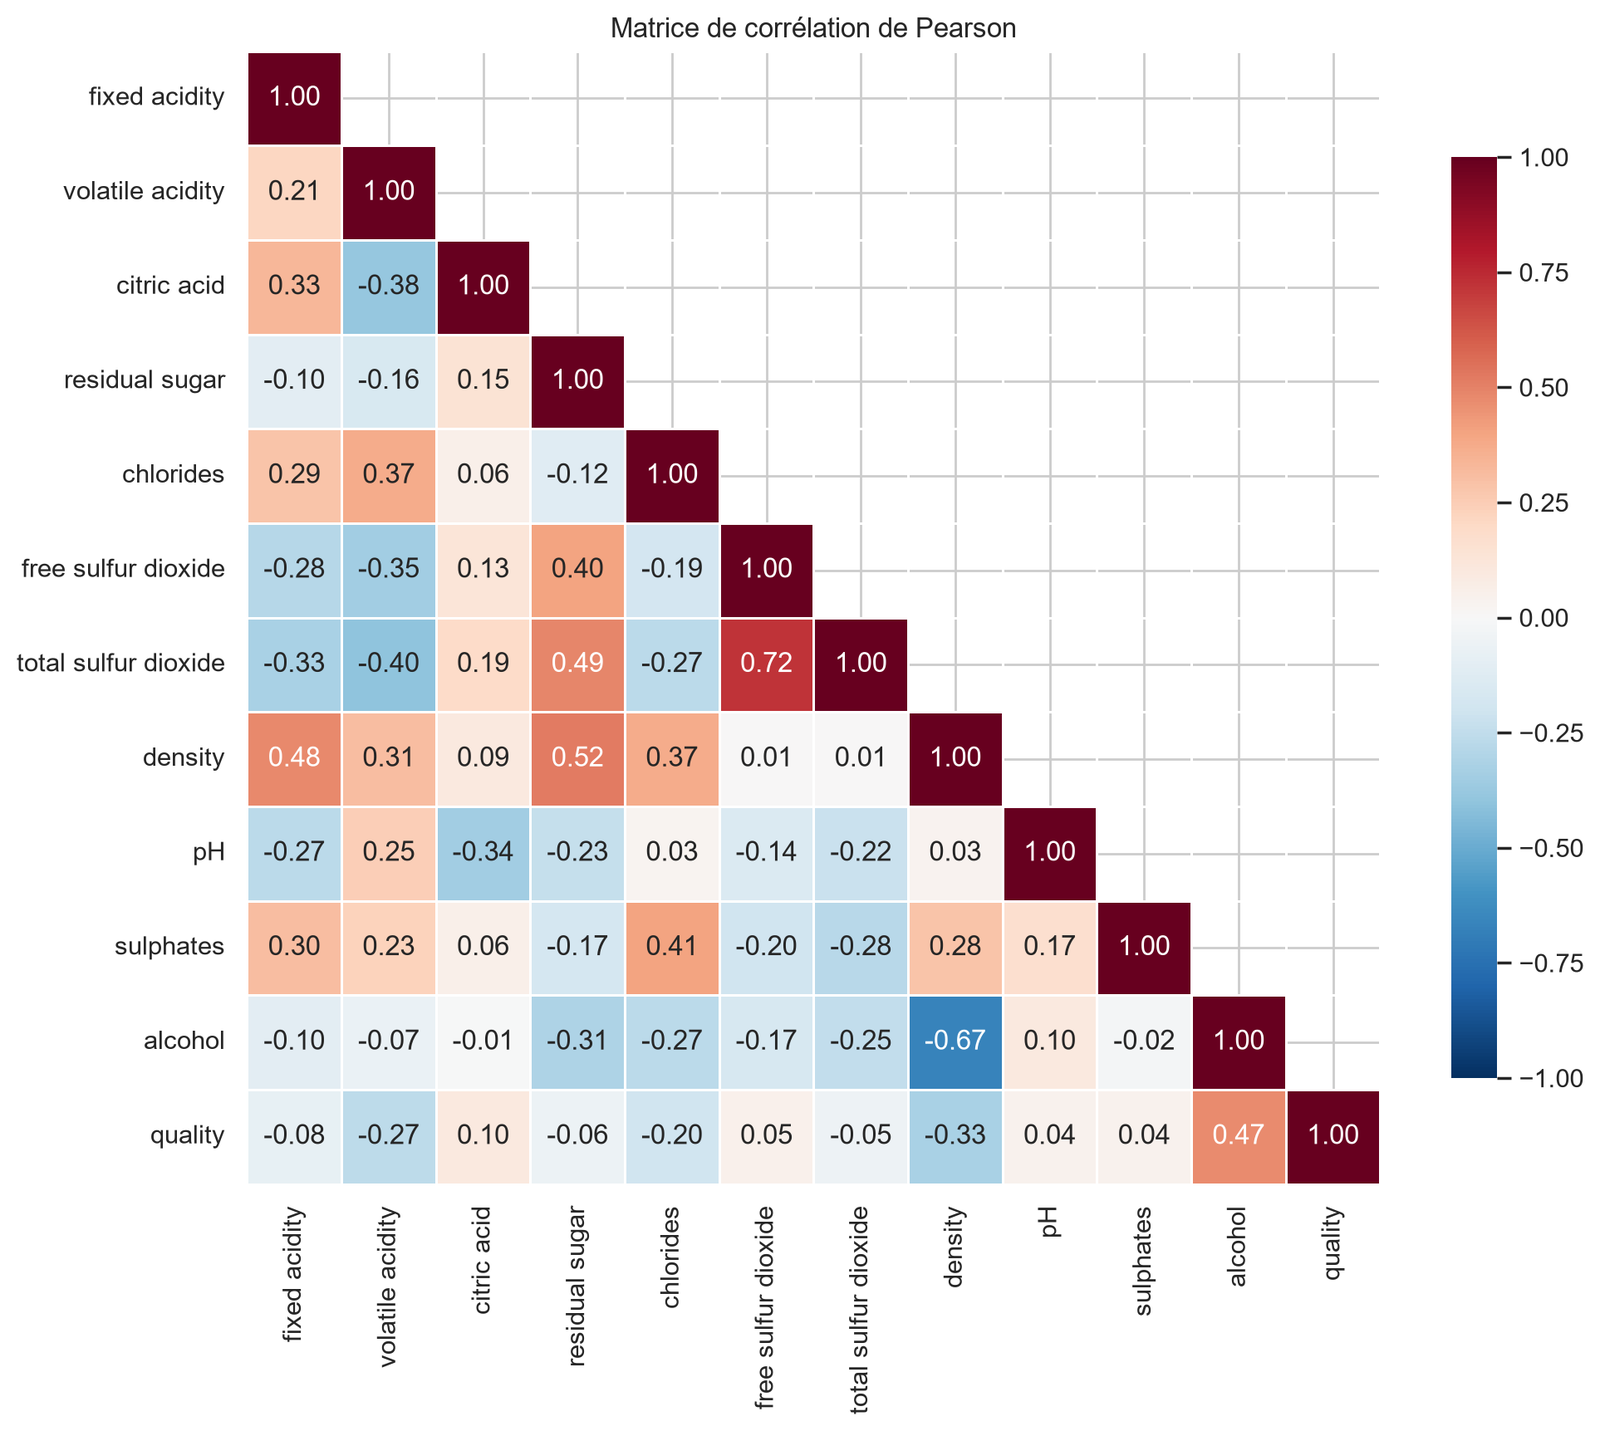
\includegraphics[width=0.85\linewidth]{04_correlation_matrix.png}
\caption{Matrice de corrélation de Pearson entre les variables et la note.}\label{fig:corr}
\end{figure}

\subsection{Lien entre les variables et la cible}

La figure~\ref{fig:boxclass} compare la distribution de chaque variable selon la classe. L'\textbf{alcool} est de loin la variable la plus discriminante
(corrélation point-bisériale $r = 0{,}42$ ; $11{,}6\,\%$ vol. en moyenne pour les bons vins contre $10{,}3\,\%$), suivi de la densité ($r = -0{,}30$)
et des chlorures ($r = -0{,}16$) ; l'acidité volatile ($r = -0{,}14$) ressort surtout par la corrélation linéaire. Les bons vins ont en moyenne plus d'alcool,
moins d'acidité volatile et moins de chlorures. Les tests de Mann-Whitney sont significatifs pour presque toutes les variables, mais l'information mutuelle
(figure~\ref{fig:mi}) montre que les sulfates, le SO$_2$ libre, l'acidité fixe et le pH apportent très peu d'information \emph{individuellement}.

\begin{figure}[htbp]
\centering
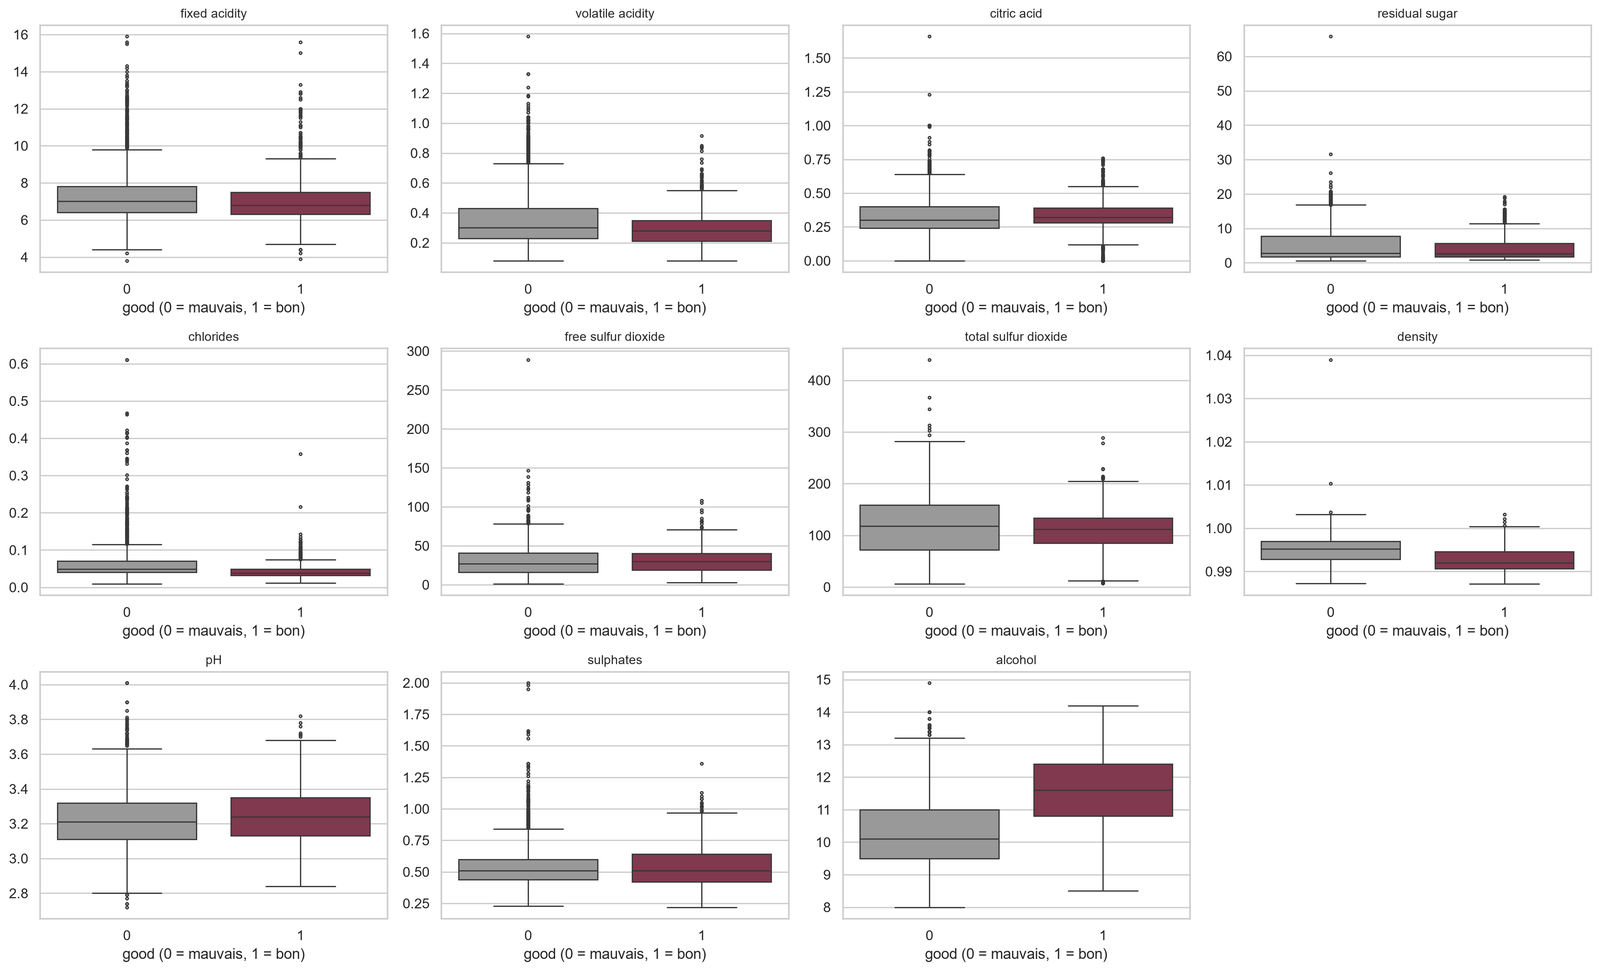
\includegraphics[width=\linewidth]{05_boxplots_by_class.png}
\caption{Distribution de chaque variable selon la classe (0 = mauvais, 1 = bon).}\label{fig:boxclass}
\end{figure}

\begin{figure}[htbp]
\centering
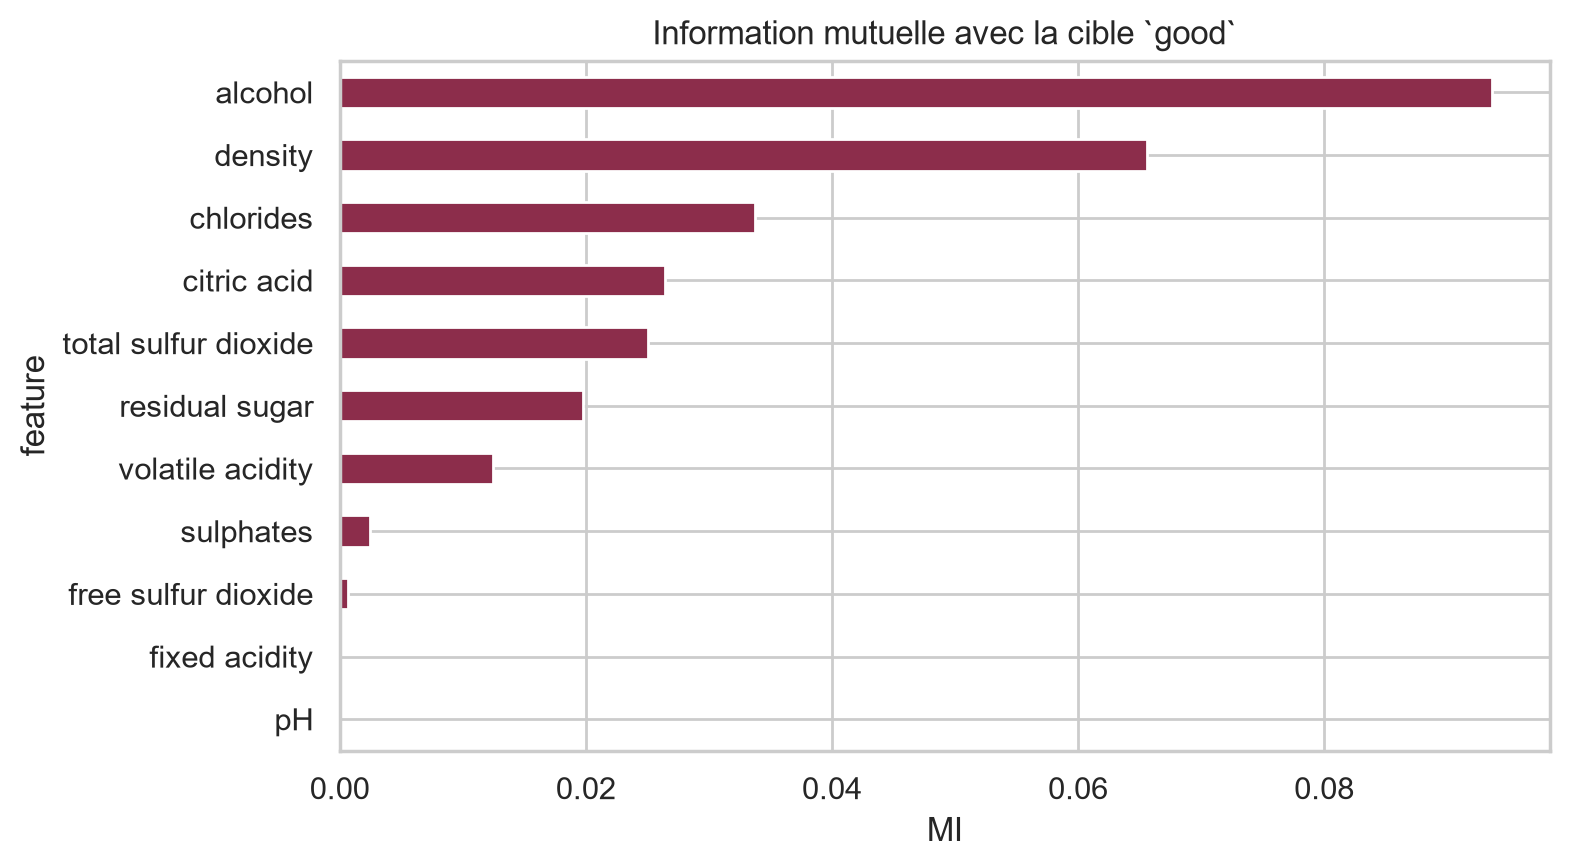
\includegraphics[width=0.6\linewidth]{06_mutual_information.png}
\caption{Information mutuelle entre chaque variable et la cible.}\label{fig:mi}
\end{figure}

\subsection{Effet du type de vin}

Les vins rouges et blancs diffèrent fortement (figure~\ref{fig:type}) : les blancs contiennent environ 2,9 fois plus de SO$_2$ total, 2,3 fois plus de sucre résiduel,
et moins d'acidité volatile et de chlorures. De plus, la force du lien variable--cible varie selon le type : la corrélation de l'acidité volatile avec la cible est
de $-0{,}27$ pour les rouges mais de seulement $-0{,}06$ pour les blancs. La variable \texttt{type} est encodée par une indicatrice binaire (\texttt{type\_white})
et un modèle capable de capter des interactions est attendu.

\begin{figure}[htbp]
\centering
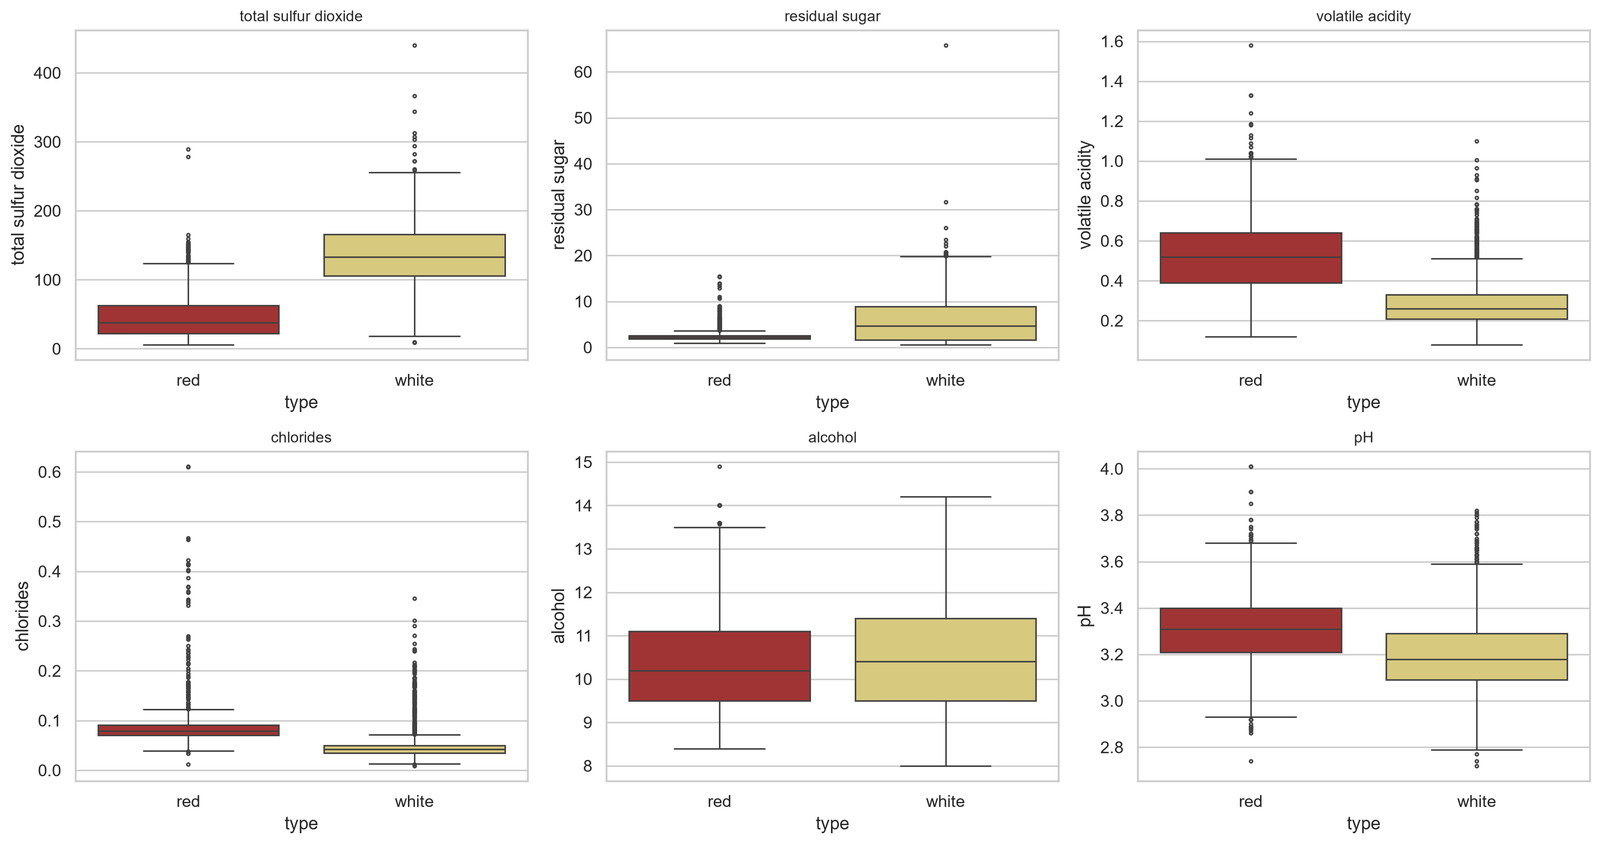
\includegraphics[width=\linewidth]{07_features_by_type.png}
\caption{Distribution de six variables selon le type de vin.}\label{fig:type}
\end{figure}

\subsection{Synthèse des décisions de prétraitement}

\begin{table}[htbp]
\centering\small
\caption{Constats de l'analyse exploratoire et décisions associées.}
\begin{tabular}{@{}p{5.2cm}p{9.5cm}@{}}
\toprule
Constat & Décision \\
\midrule
Aucune valeur manquante & Pas d'imputation \\
18\,\% de doublons exacts & Suppression avant le découpage (évite la fuite train/test) \\
Classes déséquilibrées (81\,/\,19) & Découpage stratifié, métriques F1 / ROC-AUC / AP, pondération des classes, réglage du seuil \\
Échelles hétérogènes & \texttt{StandardScaler} dans un \texttt{Pipeline} (ajusté sur le train de chaque pli) \\
Asymétrie et aberrations plausibles & Conservées ; transformation $\log(1+x)$ en option ; modèles robustes \\
Multicolinéarité (densité, SO$_2$) & Étude de la sélection de variables (VIF, L1) et régularisation \\
\texttt{type} catégorielle & Indicatrice binaire \texttt{type\_white} \\
\bottomrule
\end{tabular}
\end{table}

\paragraph{Découpage.}
Les $5\,320$ vins sont séparés en $4\,256$ vins d'entraînement (80\,\%) et $1\,064$ vins de test (20\,\%), avec stratification conjointe sur la cible et le type.
La proportion de bons vins est de 19\,\% dans les deux ensembles.

%% ------------------------------------------------------------------
\section{Sélection de variables}\label{sec:selection}

Nous comparons quatre méthodes, chacune intégrée au pipeline (donc réestimée dans chaque pli) :
\begin{itemize}
  \item \textbf{filtre par VIF} : suppression itérative de la variable de plus fort VIF tant qu'il dépasse 10 (méthode de filtrage) ;
  \item \textbf{pénalisation L1 (Lasso)} : une régression logistique $\ell_1$ ne retient que les variables de coefficient non nul (méthode intégrée), la régularisation
        $\ell_1$ étant vue en cours pour limiter le sur-apprentissage ;
  \item \textbf{importance par forêt aléatoire} : conservation des variables dont l'importance dépasse la moyenne (méthode intégrée par les arbres) ;
  \item \textbf{information mutuelle} : conservation des six variables de plus forte information mutuelle avec la cible (méthode de filtrage univariée).
\end{itemize}

Le VIF retire uniquement la densité. La pénalisation L1 ($C = 0{,}05$) ne retire que \texttt{type\_white}. Les variables \texttt{alcohol}, \texttt{chlorides} et
\texttt{total sulfur dioxide} sont retenues par les quatre méthodes.

Nous comparons les performances de trois modèles (régression logistique, SVM, forêt) selon la méthode de sélection (tableau~\ref{tab:selection}, figure~\ref{fig:selection}).

\begin{table}[htbp]
\centering\small
\caption{F1-score et ROC-AUC en validation croisée (5 plis) selon la sélection de variables. « log1p » désigne la transformation $\log(1+x)$ des variables asymétriques sans sélection.}\label{tab:selection}
\begin{tabular}{@{}lcccccc@{}}
\toprule
 & \multicolumn{3}{c}{F1} & \multicolumn{3}{c}{ROC-AUC} \\
\cmidrule(lr){2-4}\cmidrule(lr){5-7}
Sélection & Rég. log. & SVM & Forêt & Rég. log. & SVM & Forêt \\
\midrule
Aucune          & 0,532 & 0,541 & 0,556 & 0,828 & 0,845 & 0,855 \\
VIF             & 0,530 & 0,541 & 0,560 & 0,824 & 0,842 & 0,856 \\
L1              & 0,531 & 0,541 & 0,559 & 0,826 & 0,844 & 0,854 \\
Importance forêt & 0,516 & 0,510 & 0,481 & 0,811 & 0,807 & 0,808 \\
Info. mutuelle  & 0,517 & 0,516 & 0,523 & 0,805 & 0,809 & 0,819 \\
log1p           & 0,538 & 0,540 & 0,557 & 0,832 & 0,846 & 0,854 \\
\bottomrule
\end{tabular}
\end{table}

\begin{figure}[htbp]
\centering
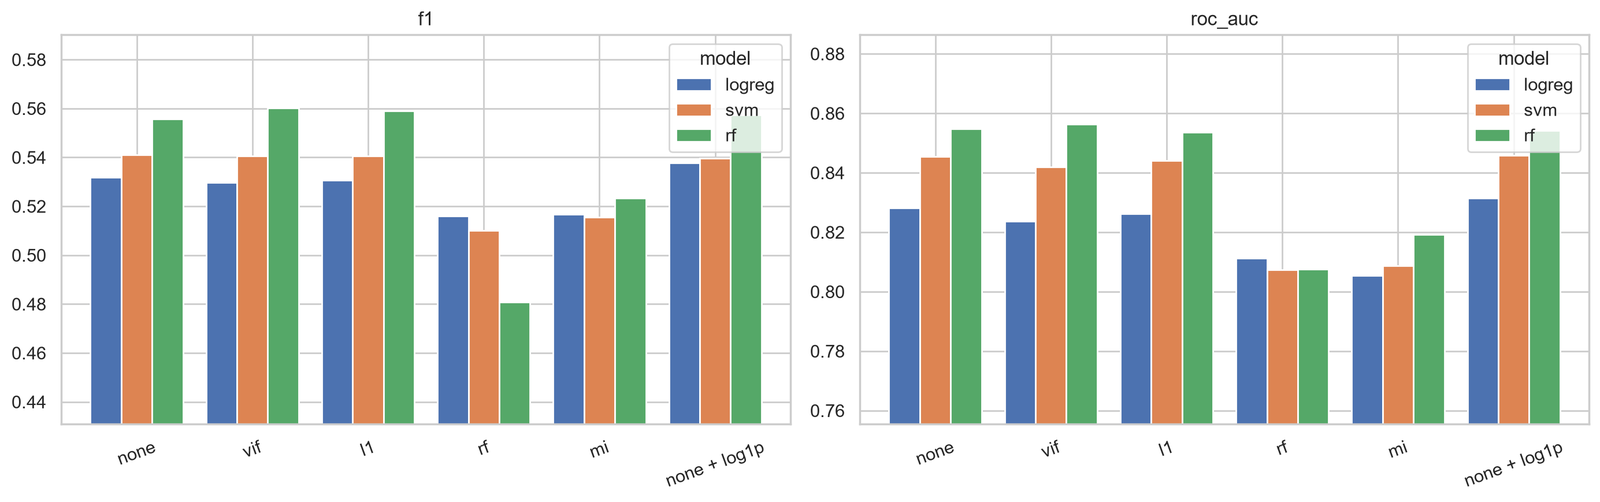
\includegraphics[width=\linewidth]{08_selection_comparison.png}
\caption{Effet de la sélection de variables sur le F1 et le ROC-AUC.}\label{fig:selection}
\end{figure}

\paragraph{Résultats.}
Les filtres VIF et L1 donnent des performances \emph{identiques} à l'absence de sélection (écarts $\leq 0{,}005$, inférieurs à l'écart-type entre plis) :
on peut réduire la multicolinéarité sans perte. À l'inverse, la sélection par importance de forêt (seuil à la moyenne) et par information mutuelle
(six variables) éliminent trop d'information et \textbf{dégradent} nettement les scores ; l'information mutuelle, purement univariée, ignore les variables utiles
seulement en combinaison (par exemple l'acidité volatile). La transformation $\log(1+x)$ n'apporte qu'un gain marginal pour la régression logistique ($+0{,}006$ de F1) et rien pour la forêt.
Nous ne retenons donc aucune sélection destructive : le choix entre « aucune » et « VIF » ainsi que l'option $\log(1+x)$ sont laissés à la recherche d'hyperparamètres (section~\ref{sec:tuning}).

%% ------------------------------------------------------------------
\section{Choix et justification des modèles}\label{sec:modeles}

Nous étudions les cinq modèles de l'énoncé, auxquels nous ajoutons une baseline triviale (\texttt{DummyClassifier}, classe majoritaire) et deux méthodes d'ensemble vues en cours
(forêt aléatoire, \emph{gradient boosting}) comme points de comparaison. Le choix s'appuie sur leurs propriétés théoriques (linéaire contre non linéaire, hypothèses de distribution,
sensibilité à l'échelle) et sur l'adéquation aux données observées (variables continues, corrélées, asymétriques et bruitées ; labels issus de jurys humains), résumés dans le tableau~\ref{tab:modeles}.

\begin{table}[htbp]
\centering\scriptsize
\caption{Propriétés théoriques des modèles comparés.}\label{tab:modeles}
\begin{tabular}{@{}p{2.1cm}p{3.1cm}p{2.7cm}p{2.3cm}p{4.3cm}@{}}
\toprule
Modèle & Famille & Frontière & Échelle & Limites principales \\
\midrule
Régression logistique & Linéaire, discriminatif & Hyperplan & Sensible & Frontière linéaire ; instable si variables colinéaires \\
$k$-NN & Non paramétrique, distance & Non linéaire, locale & Très sensible & Bruit, variables non pertinentes ; $k$ à valider \\
Arbre de décision & Règles (Gini, entropie) & Rectangles alignés sur les axes & Indifférent & Variance élevée, sur-apprentissage \\
Naive Bayes & Probabiliste génératif & Quadratique & Indifférent & Indépendance et gaussianité violées ici \\
SVM (RBF) & Marge maximale, à noyau & Non linéaire & Très sensible & $C$ et $\gamma$ à régler ; peu interprétable \\
Forêt aléatoire & Bagging d'arbres & Non linéaire & Indifférent & Moins interprétable, volumineux \\
Gradient boosting & Boosting d'arbres & Non linéaire & Indifférent & Sensible au bruit et aux hyperparamètres \\
\bottomrule
\end{tabular}
\end{table}

\paragraph{Modèles linéaires et paramétriques.}
La \textbf{régression logistique} modélise $P(y=1\mid x) = \sigma(w^\top x + b)$ ; elle est rapide, ses coefficients sont interprétables, mais sa frontière est un hyperplan et
elle souffre de la multicolinéarité observée en section~\ref{sec:data}. \textbf{Naive Bayes} suppose l'indépendance conditionnelle des variables et, ici, des lois gaussiennes :
\begin{equation}
  P(y \mid x) \propto P(y) \prod_{j=1}^{11} \mathcal{N}(x_j \mid \mu_{j,y}, \sigma_{j,y}^2).
\end{equation}
Cette hypothèse est mise à mal par les corrélations (SO$_2$, alcool--densité) et les asymétries : nous nous attendons à de moins bonnes performances.

\paragraph{Modèles non linéaires.}
Le \textbf{$k$-NN} classe un point par vote de ses $k$ plus proches voisins ; un petit $k$ donne un biais faible et une variance élevée, un grand $k$ l'inverse. Il exige la standardisation
des variables. L'\textbf{arbre de décision} partitionne l'espace selon un critère d'impureté (Gini ou entropie) : interprétable et robuste aux aberrations, mais de variance élevée. Le \textbf{SVM à noyau RBF}
cherche l'hyperplan de marge maximale dans un espace transformé par
\begin{equation}
  K(x, x') = \exp\!\big(-\gamma \lVert x - x'\rVert^2\big),
\end{equation}
avec une marge souple contrôlée par $C$, robuste au bruit. La \textbf{forêt aléatoire}~\cite{breiman2001} moyenne de nombreux arbres construits sur des échantillons bootstrap et des sous-ensembles
aléatoires de variables (réduction de la variance) ; le \textbf{boosting} construit séquentiellement des arbres qui corrigent les erreurs des précédents (réduction du biais).

Le déséquilibre des classes est pris en compte par \texttt{class\_weight=balanced} pour les modèles qui le supportent (régression logistique, arbre, SVM, forêt).

%% ------------------------------------------------------------------
\section{Évaluation des modèles}\label{sec:eval}

\subsection{Métriques et protocole}

Pour la classe positive (bon vin), nous calculons la précision $P = \frac{TP}{TP+FP}$, le rappel $R = \frac{TP}{TP+FN}$ et le F1-score $F_1 = \frac{2PR}{P+R}$, ainsi que
l'accuracy, la matrice de confusion, la courbe ROC et son aire (AUC), et la courbe précision-rappel (AP). L'AUC et l'AP ne dépendent pas du seuil de décision ; le F1, la précision
et le rappel dépendent de ce seuil, initialement fixé à $0{,}5$.

Les modèles sont comparés par \textbf{validation croisée stratifiée à 5 plis} sur le jeu d'entraînement. Les figures de confusion, ROC et PR sont calculées à partir de
\textbf{prédictions hors-pli} : chaque vin est noté par un modèle qui ne l'a pas vu à l'entraînement.

\subsection{Résultats avec les réglages par défaut}

\begin{table}[htbp]
\centering\small
\caption{Validation croisée à 5 plis, réglages par défaut (moyenne $\pm$ écart-type entre plis ; classe positive pour précision, rappel et F1).}\label{tab:default}
\begin{tabular}{@{}lccccccc@{}}
\toprule
Modèle & Accuracy & Précision & Rappel & F1 & ROC-AUC & AP & F1 train \\
\midrule
Dummy        & 0,810 & 0,000 & 0,000 & 0,000 & 0,500 & 0,190 & 0,000 \\
Rég. log.    & 0,737 & 0,403 & 0,784 & 0,532 & 0,828 & 0,509 & 0,537 \\
$k$-NN       & 0,830 & 0,567 & 0,434 & 0,491 & 0,799 & 0,469 & 0,635 \\
Arbre        & 0,789 & 0,442 & 0,429 & 0,435 & 0,651 & 0,298 & 1,000 \\
Naive Bayes  & 0,745 & 0,395 & 0,646 & 0,490 & 0,769 & 0,446 & 0,490 \\
SVM (RBF)    & 0,740 & 0,407 & 0,808 & 0,541 & 0,845 & 0,539 & 0,585 \\
Forêt        & 0,826 & 0,540 & 0,574 & 0,556 & 0,855 & 0,592 & 0,997 \\
Boosting     & 0,833 & 0,610 & 0,340 & 0,434 & 0,843 & 0,539 & 0,597 \\
\bottomrule
\end{tabular}
\end{table}

\begin{figure}[htbp]
\centering
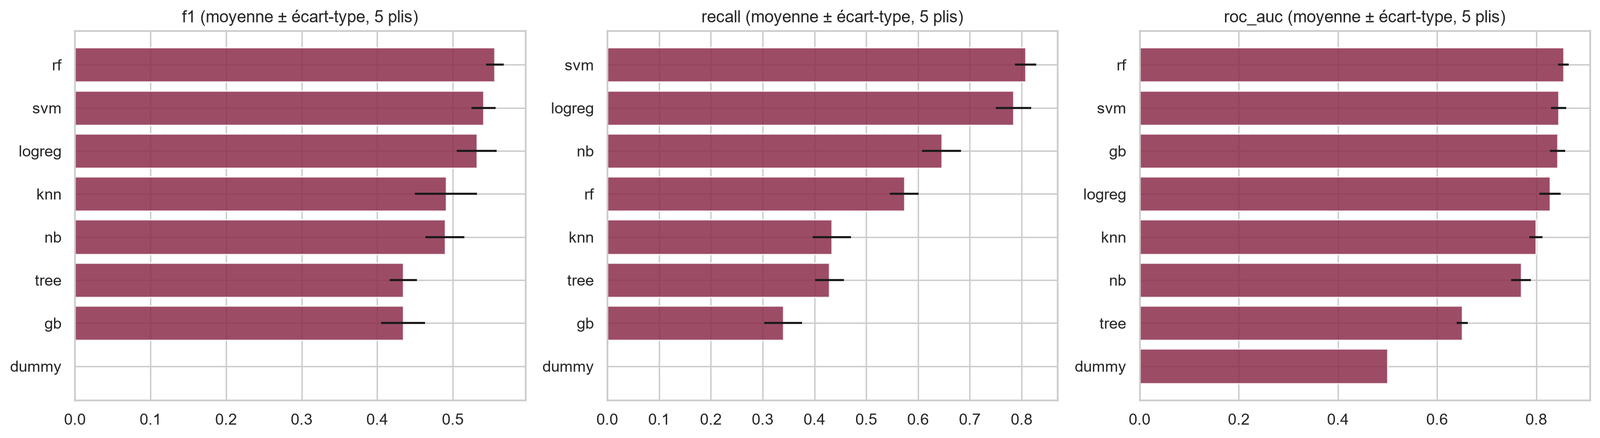
\includegraphics[width=\linewidth]{09_models_cv_comparison.png}
\caption{Comparaison des modèles par défaut : F1, rappel et ROC-AUC (moyenne $\pm$ écart-type, 5 plis).}\label{fig:cvcomp}
\end{figure}

\paragraph{Interprétation (figure~\ref{fig:cvcomp}).}
\begin{itemize}
  \item La baseline atteint 81\,\% d'accuracy avec un rappel nul : l'\textbf{accuracy est trompeuse} sur des classes 80/20.
  \item La \textbf{forêt} a les meilleurs F1 ($0{,}556$) et ROC-AUC ($0{,}855$), mais elle sur-apprend fortement (F1 d'entraînement $\approx 1$).
  \item Le \textbf{SVM} et la \textbf{régression logistique} pondérés par classe ont le meilleur rappel ($0{,}81$ et $0{,}78$) au prix d'une précision d'environ $0{,}40$.
  \item Le \textbf{boosting} et le \textbf{$k$-NN} ont la meilleure précision ($0{,}61$ et $0{,}57$) mais un rappel faible ($0{,}34$ et $0{,}43$) : ils prédisent peu de bons vins. Le ROC-AUC
        du boosting ($0{,}843$) montre que son \emph{classement} est bon : c'est le seuil à $0{,}5$ qui est mal placé.
  \item L'\textbf{arbre seul} est le moins bon modèle non trivial (AUC $0{,}651$), typique d'une variance élevée ; \textbf{Naive Bayes} (AUC $0{,}769$) est pénalisé par la corrélation des variables.
\end{itemize}

\begin{figure}[htbp]
\centering
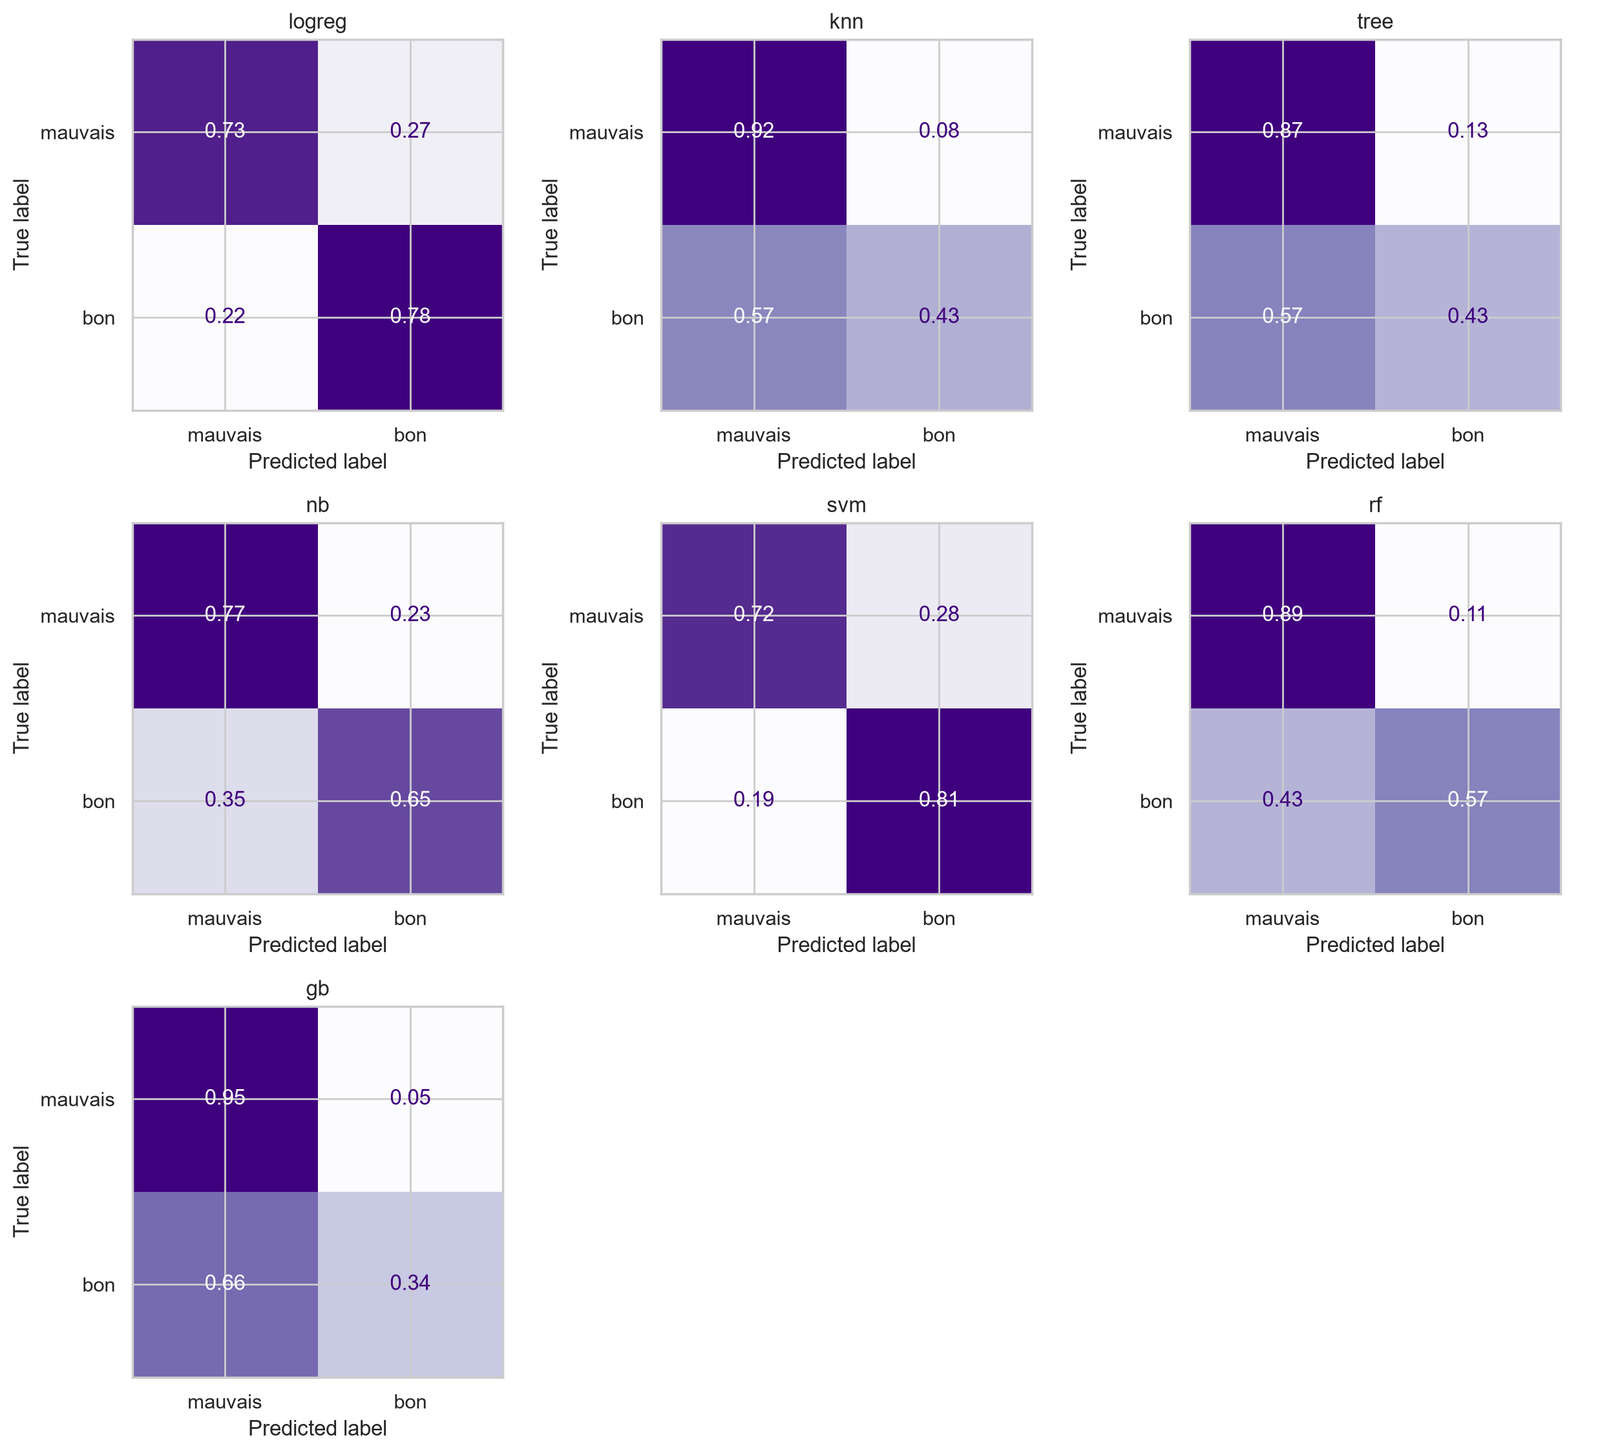
\includegraphics[width=\linewidth]{10_confusion_matrices.png}
\caption{Matrices de confusion hors-pli (normalisées par ligne) au seuil par défaut.}\label{fig:conf}
\end{figure}

\begin{figure}[htbp]
\centering
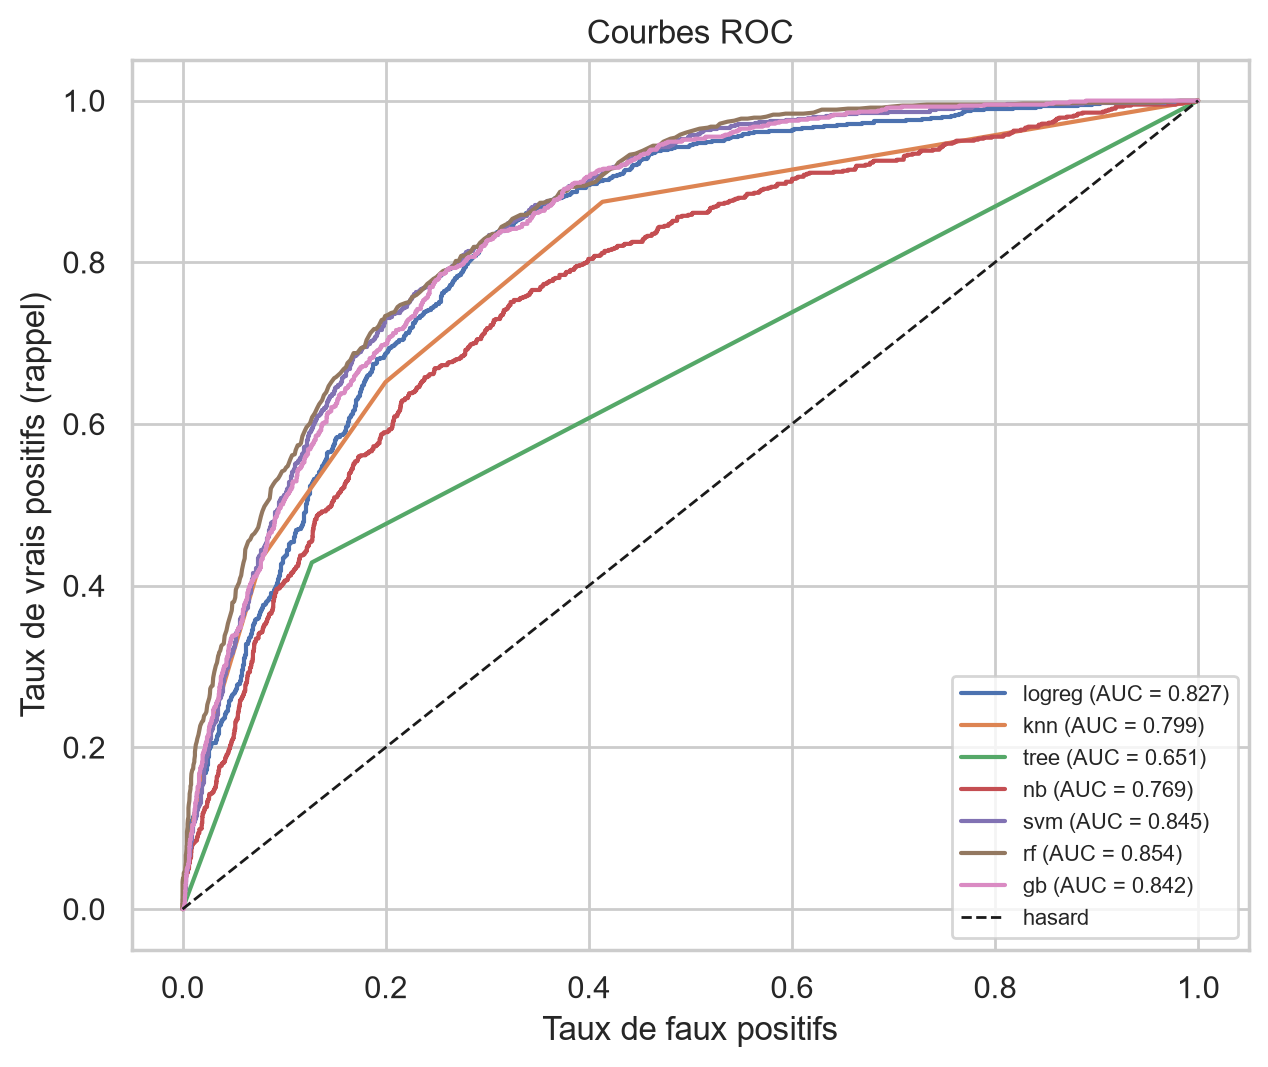
\includegraphics[width=0.75\linewidth]{11_roc_curves.png}
\caption{Courbes ROC hors-pli des modèles par défaut.}\label{fig:roc}
\end{figure}

\begin{figure}[htbp]
\centering
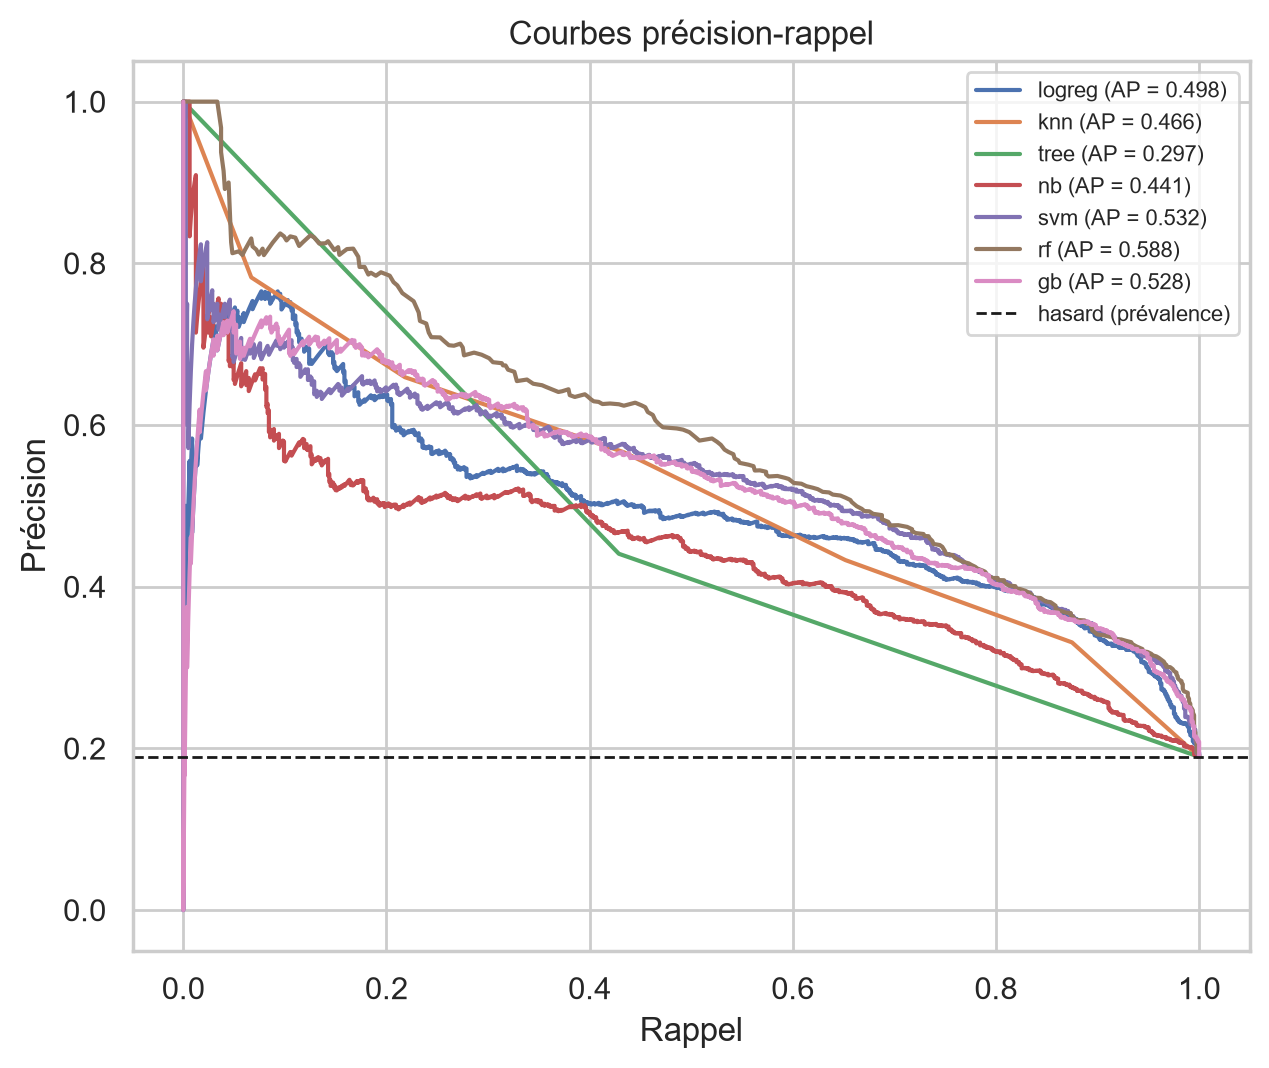
\includegraphics[width=0.75\linewidth]{12_pr_curves.png}
\caption{Courbes précision-rappel hors-pli des modèles par défaut.}\label{fig:pr}
\end{figure}

Les matrices de confusion (figure~\ref{fig:conf}) montrent le compromis rappel/spécificité : le SVM détecte 81\,\% des bons vins (72\,\% des mauvais bien classés) et la régression logistique
78\,\% (73\,\%), tandis que le boosting (34\,\% / 95\,\%) et le $k$-NN (43\,\% / 92\,\%) privilégient la spécificité. Les courbes ROC et PR (figures~\ref{fig:roc} et~\ref{fig:pr}) ne dépendent pas du seuil et classent
la forêt, le SVM et le boosting en tête. Pour un problème déséquilibré, la courbe PR est plus informative : l'AP de la forêt ($0{,}59$) est très supérieure à la prévalence ($0{,}19$).

\subsection{Compromis biais/variance}

Le tableau~\ref{tab:default} (colonne « F1 train ») et les courbes d'apprentissage (figure~\ref{fig:learning}) permettent de diagnostiquer le biais et la variance :
\begin{itemize}
  \item \textbf{Arbre et forêt} : F1 d'entraînement $\approx 1$ contre $0{,}44$ et $0{,}56$ en validation : \textbf{variance élevée} (sur-apprentissage). Les courbes ne se rejoignent pas ;
        plus de régularisation (profondeur, \texttt{min\_samples\_leaf}) est nécessaire.
  \item \textbf{Régression logistique et Naive Bayes} : courbes d'entraînement et de validation confondues et basses : \textbf{biais élevé} (sous-apprentissage). Ajouter des données n'aiderait pas ;
        il faut des modèles plus expressifs.
  \item \textbf{SVM RBF} : bon compromis (écart train/validation $\approx 0{,}04$).
  \item \textbf{$k$-NN} : écart notable ($0{,}64$ contre $0{,}49$) ; le choix de $k$ pilote le compromis (figure~\ref{fig:complex}).
\end{itemize}
Dans la figure~\ref{fig:complex}, la meilleure profondeur d'arbre se situe autour de $3$ (F1 $\approx 0{,}51$), puis la validation se dégrade alors que l'entraînement monte.
Pour le $k$-NN, le F1 de validation \emph{baisse} quand $k$ augmente, car avec un vote majoritaire non pondéré un grand $k$ prédit presque toujours la classe majoritaire ; le meilleur $k$ dépend donc
du seuil et de la métrique optimisés.

\begin{figure}[htbp]
\centering
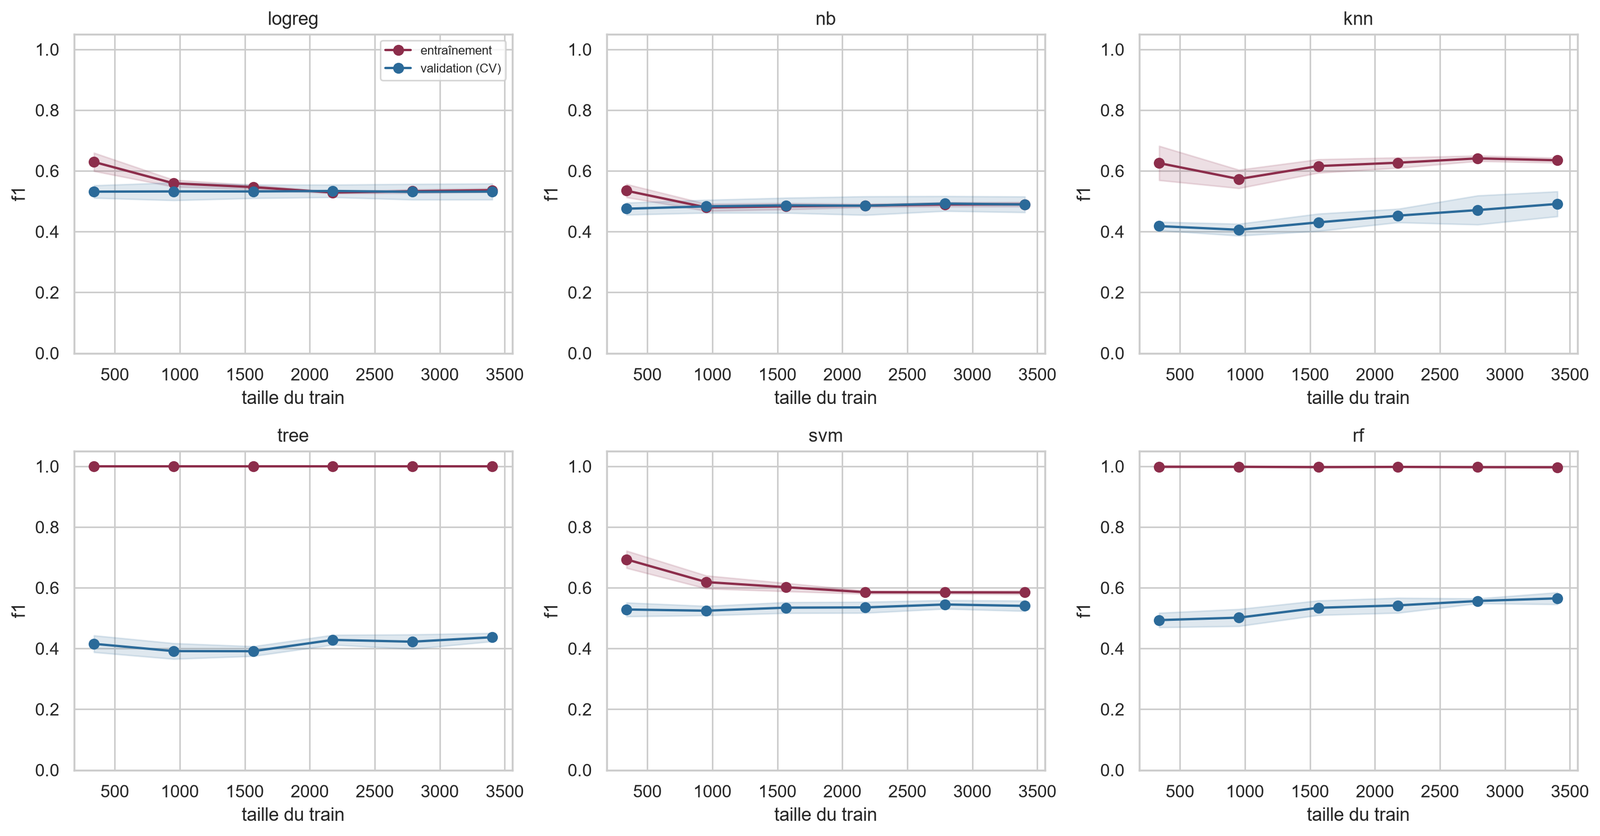
\includegraphics[width=\linewidth]{13_learning_curves.png}
\caption{Courbes d'apprentissage (F1 d'entraînement et de validation selon la taille du train).}\label{fig:learning}
\end{figure}

\begin{figure}[htbp]
\centering
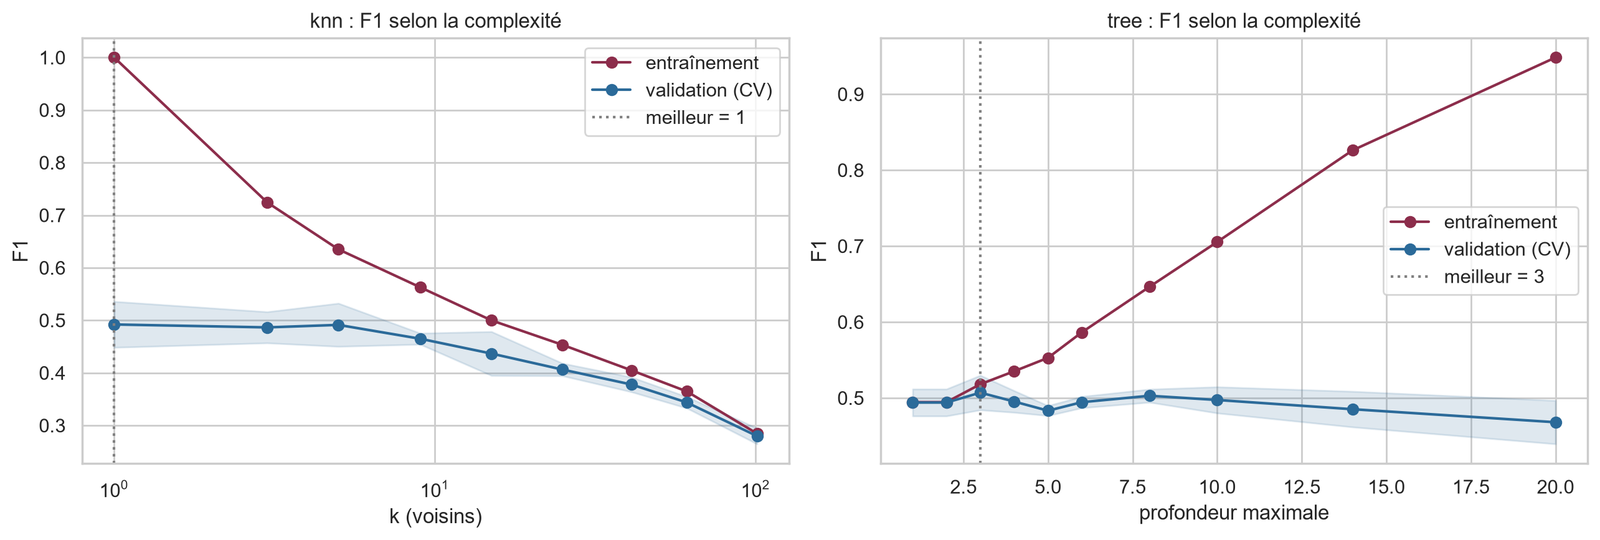
\includegraphics[width=\linewidth]{14_complexity_curves.png}
\caption{Complexité contre performance : $k$ pour le $k$-NN et profondeur maximale pour l'arbre.}\label{fig:complex}
\end{figure}

%% ------------------------------------------------------------------
\section{Optimisation des hyperparamètres}\label{sec:tuning}

\subsection{Protocole}

L'optimisation se fait en validation croisée stratifiée à 5 plis sur le jeu d'entraînement, avec le \textbf{ROC-AUC} comme critère (indépendant du seuil et adapté aux classes déséquilibrées).
Le prétraitement (\texttt{std} ou $\log(1+x)$) et la sélection (aucune ou VIF) font partie de l'espace de recherche. Nous utilisons :
\begin{itemize}
  \item le \textbf{Grid Search} (recherche exhaustive) pour les modèles à peu d'hyperparamètres : régression logistique ($C$, pondération), $k$-NN ($k$, pondération des voisins, distance $L_1$ ou $L_2$),
        arbre (profondeur, \texttt{min\_samples\_leaf}, critère), Naive Bayes (\texttt{var\_smoothing}) ;
  \item le \textbf{Random Search}~\cite{bergstra2012} (tirages aléatoires) pour les modèles à plus d'hyperparamètres : SVM (40 tirages sur $C$, $\gamma$, pondération),
        forêt (30 tirages) et boosting (30 tirages).
\end{itemize}

\subsection{Résultats}

Le tableau~\ref{tab:tuning} donne, pour chaque modèle, la méthode utilisée, le nombre de candidats et les meilleurs réglages.

\begin{table}[htbp]
\centering\small
\caption{Meilleurs réglages et ROC-AUC en validation croisée.}\label{tab:tuning}
\begin{tabular}{@{}llrp{6.3cm}@{}}
\toprule
Modèle & Méthode & AUC CV & Meilleurs hyperparamètres \\
\midrule
Forêt        & Random (30) & 0,855 & 600 arbres, \texttt{min\_samples\_leaf}=3, \texttt{max\_features}=log2, profondeur 24 \\
Boosting     & Random (30) & 0,853 & taux d'apprentissage 0,020, profondeur 5, \texttt{subsample}=0,8 \\
SVM (RBF)    & Random (40) & 0,847 & $C \approx 1{,}53$, $\gamma \approx 0{,}062$, classes pondérées \\
$k$-NN       & Grid (112)  & 0,845 & $k=41$, distance de Manhattan, vote pondéré par la distance \\
Rég. log.    & Grid (56)   & 0,832 & $C=1$, transformation $\log(1+x)$ \\
Arbre        & Grid (192)  & 0,798 & entropie, profondeur 5, \texttt{min\_samples\_leaf}=20 \\
Naive Bayes  & Grid (28)   & 0,780 & \texttt{var\_smoothing}=$10^{-3}$, $\log(1+x)$, VIF \\
\bottomrule
\end{tabular}
\end{table}

Les cinq meilleures configurations de chaque modèle sont très proches (écarts de l'ordre de $0{,}001$ d'AUC) : la surface de performance est un \emph{plateau}, pas un pic étroit,
et les résultats sont peu sensibles au réglage fin. Les choix structurels (\texttt{std} ou $\log(1+x)$, aucune sélection ou VIF) ont peu d'effet ; la régression logistique et Naive Bayes
préfèrent $\log(1+x)$, et la suppression de la densité par le VIF ne coûte rien.

\subsection{Grid Search contre Random Search : coût et gain}

Pour le SVM, nous comparons une grille $7 \times 5$ sur $(C, \gamma)$ à des tirages aléatoires dans les mêmes intervalles (tableau~\ref{tab:gridrandom}).
À budget égal (35 candidats), les deux méthodes donnent le même résultat. Avec 20 tirages, le Random Search atteint $0{,}8465$ en 42\,\% de temps en moins que la grille pour une perte de $0{,}0002$ d'AUC ;
avec 10 tirages la perte est de $0{,}0026$, inférieure à l'écart-type entre plis. Le coût d'une grille croît exponentiellement avec le nombre d'hyperparamètres alors que celui du Random Search est fixé par le nombre de tirages ;
la grille est donc réservée aux modèles à un à trois hyperparamètres.

\begin{table}[htbp]
\centering\small
\caption{Grid Search et Random Search sur le SVM.}\label{tab:gridrandom}
\begin{tabular}{@{}lrrr@{}}
\toprule
Méthode & Candidats & Durée (s) & ROC-AUC CV \\
\midrule
Grid $7\times5$ & 35 & 3,9 & 0,8467 \\
Random 10       & 10 & 1,3 & 0,8441 \\
Random 20       & 20 & 2,3 & 0,8465 \\
Random 35       & 35 & 3,9 & 0,8465 \\
\bottomrule
\end{tabular}
\end{table}

La carte de chaleur de la figure~\ref{fig:heat} montre une \textbf{crête diagonale} : un $C$ élevé doit être compensé par un $\gamma$ faible ($C \approx 35$ avec $\gamma \approx 0{,}01$ donne la même AUC que $C \approx 1{,}5$ avec $\gamma \approx 0{,}06$).
Le coin $C$ grand / $\gamma$ grand (AUC $0{,}770$) correspond au sur-apprentissage (frontière trop flexible), et le coin $C$ petit / $\gamma$ petit ($0{,}809$) au sous-apprentissage.

\begin{figure}[htbp]
\centering
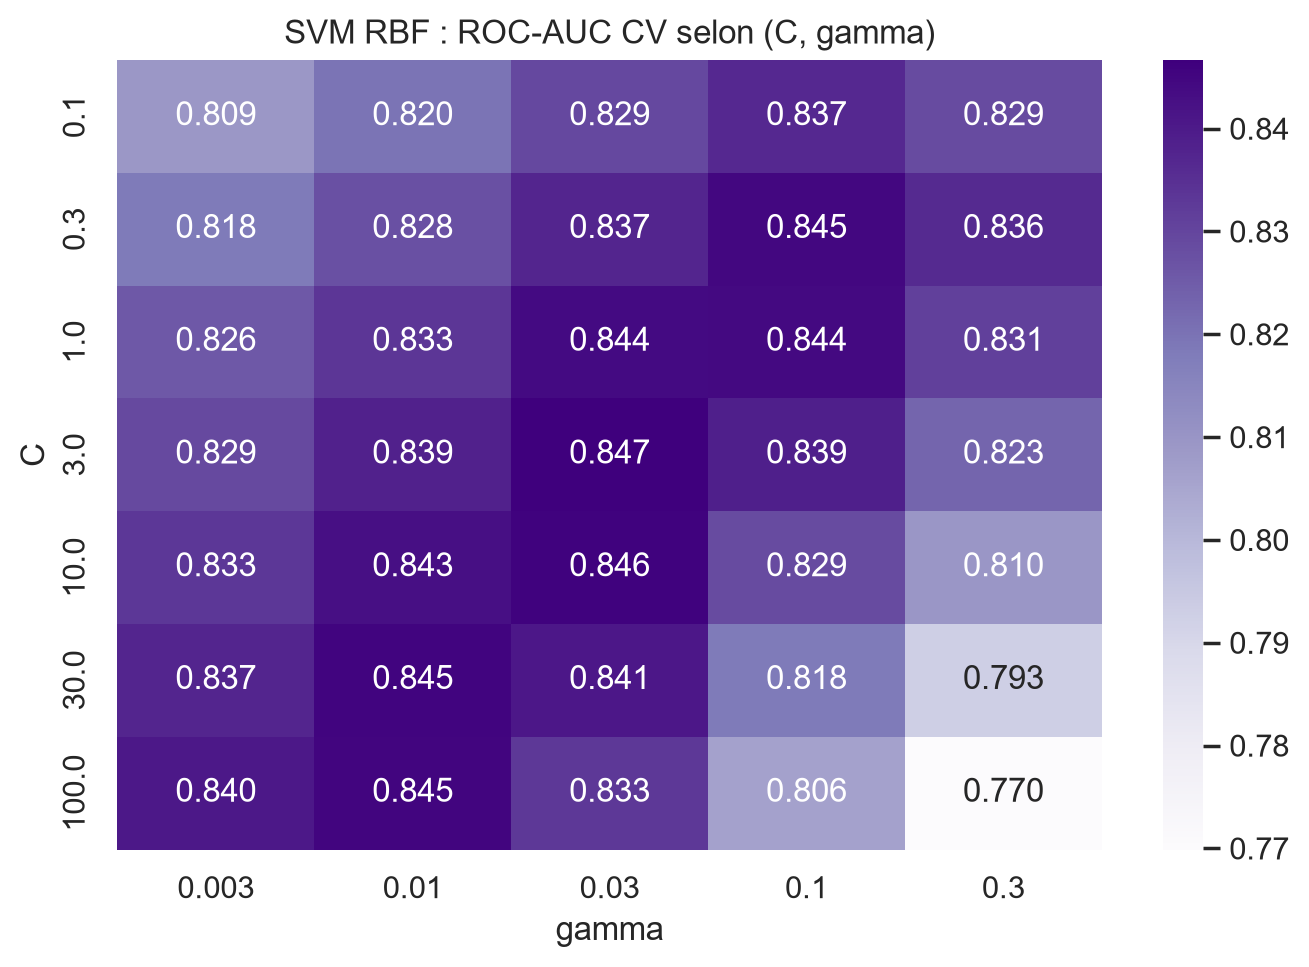
\includegraphics[width=0.7\linewidth]{15_svm_grid_heatmap.png}
\caption{ROC-AUC en validation croisée du SVM selon $(C, \gamma)$.}\label{fig:heat}
\end{figure}

\subsection{Gain par rapport aux réglages par défaut}

\begin{table}[htbp]
\centering\small
\caption{ROC-AUC en validation croisée : réglages par défaut et optimisés.}\label{tab:gain}
\begin{tabular}{@{}lrrr@{}}
\toprule
Modèle & Défaut & Optimisé & Gain \\
\midrule
Arbre        & 0,651 & 0,798 & $+0{,}148$ \\
$k$-NN       & 0,799 & 0,845 & $+0{,}045$ \\
Naive Bayes  & 0,769 & 0,780 & $+0{,}011$ \\
Boosting     & 0,843 & 0,853 & $+0{,}010$ \\
Rég. log.    & 0,828 & 0,832 & $+0{,}004$ \\
SVM (RBF)    & 0,845 & 0,847 & $+0{,}002$ \\
Forêt        & 0,855 & 0,855 & $+0{,}000$ \\
\bottomrule
\end{tabular}
\end{table}

Le gain est important pour les modèles à forte variance ou sensibles à la géométrie (arbre : $+0{,}148$ grâce à la profondeur et à \texttt{min\_samples\_leaf} ; $k$-NN : $+0{,}045$), faible ou nul pour les autres,
dont les réglages par défaut étaient déjà proches de l'optimum (tableau~\ref{tab:gain} et figure~\ref{fig:gain}). Le plafond observé (AUC $\approx 0{,}85$) tient à l'\textbf{information contenue dans les variables} :
la note est un jugement subjectif et les mesures physico-chimiques ne l'expliquent qu'en partie.

\begin{figure}[htbp]
\centering
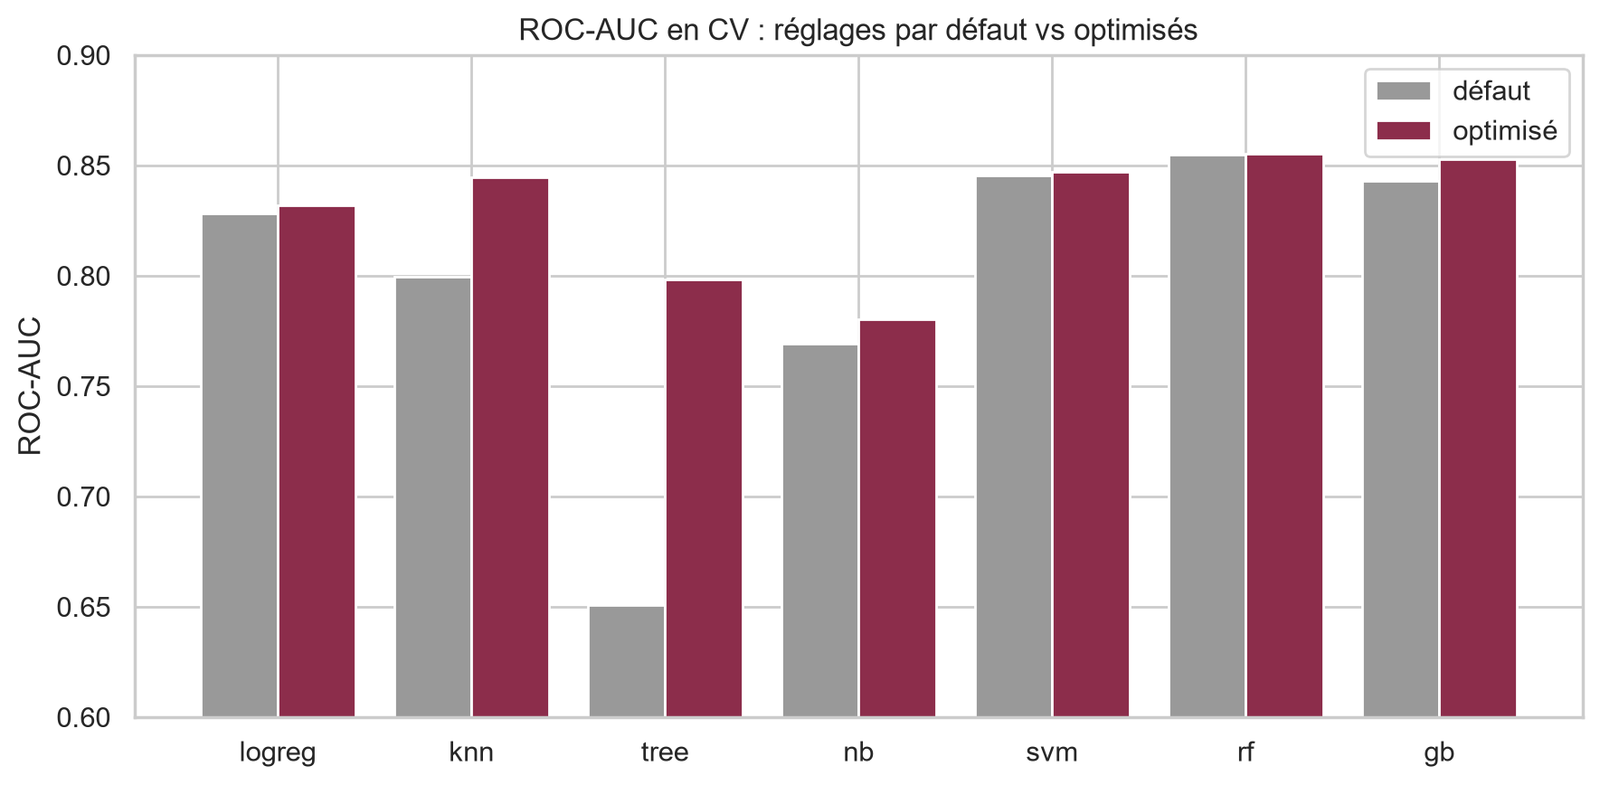
\includegraphics[width=0.75\linewidth]{16_tuning_gain.png}
\caption{ROC-AUC en validation croisée, réglages par défaut et optimisés.}\label{fig:gain}
\end{figure}

\subsection{Seuil de décision}

Le seuil $0{,}5$ n'est pas adapté à des classes 80/20. Pour chaque modèle optimisé, nous choisissons le seuil qui \textbf{maximise le F1 sur les prédictions hors-pli} du jeu d'entraînement (jamais sur le test).
Le seuil ne modifie ni l'AUC ni l'AP, seulement le compromis précision/rappel (tableau~\ref{tab:seuil}, figure~\ref{fig:prtuned}). Il apporte un gain \emph{important} aux modèles dont les scores ne sont pas calibrés pour des classes déséquilibrées : boosting
(F1 $0{,}466 \to 0{,}574$ avec un seuil de $0{,}26$), $k$-NN ($0{,}414 \to 0{,}554$) et régression logistique non pondérée ($0{,}394 \to 0{,}551$), et presque rien à la forêt et au SVM, déjà pondérés par classe.

\begin{table}[htbp]
\centering\small
\caption{Prédictions hors-pli sur le train : AUC, AP et F1 au seuil par défaut puis au seuil optimal.}\label{tab:seuil}
\begin{tabular}{@{}lcccccc@{}}
\toprule
Modèle & AUC & AP & F1 (seuil 0,5) & Seuil opt. & F1 (opt.) & Préc. / Rappel \\
\midrule
Vote souple (§\ref{sec:final}) & 0,859 & 0,587 & 0,506 & 0,343 & \textbf{0,585} & 0,494 / 0,717 \\
Forêt        & 0,855 & 0,581 & 0,571 & 0,457 & 0,575 & 0,469 / 0,742 \\
Boosting     & 0,852 & 0,562 & 0,466 & 0,264 & 0,574 & 0,483 / 0,708 \\
SVM          & 0,846 & 0,535 & 0,539 & 0,534 & 0,570 & 0,491 / 0,680 \\
$k$-NN       & 0,844 & 0,560 & 0,414 & 0,289 & 0,554 & 0,451 / 0,717 \\
Rég. log.    & 0,831 & 0,510 & 0,394 & 0,230 & 0,551 & 0,441 / 0,735 \\
Arbre        & 0,797 & 0,453 & 0,493 & 0,620 & 0,511 & 0,402 / 0,700 \\
Naive Bayes  & 0,780 & 0,461 & 0,496 & 0,419 & 0,504 & 0,408 / 0,660 \\
\bottomrule
\end{tabular}
\end{table}

\begin{figure}[htbp]
\centering
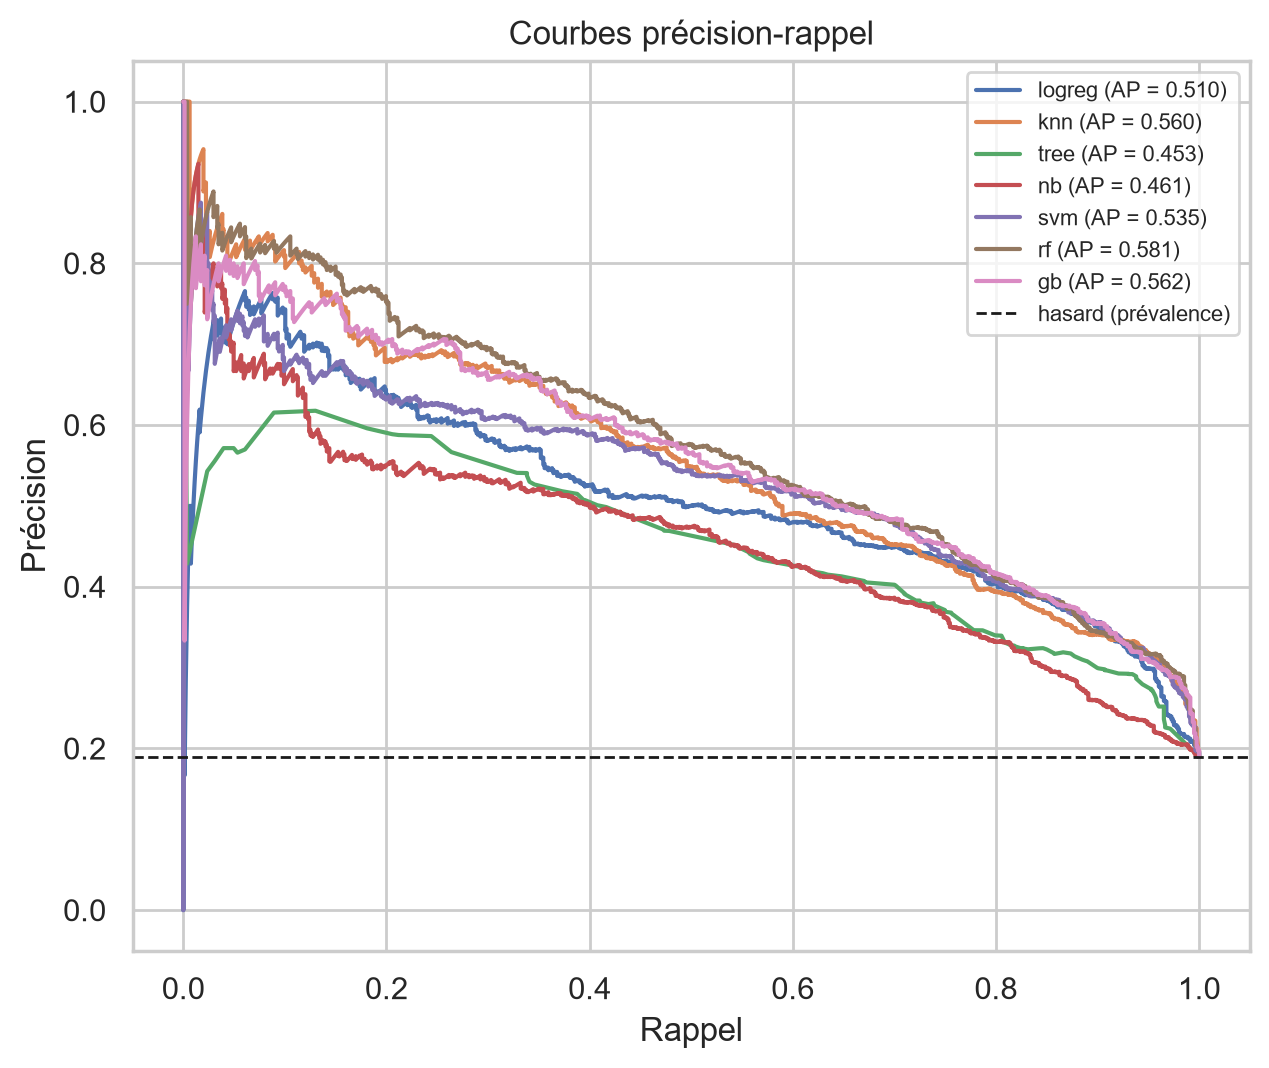
\includegraphics[width=0.75\linewidth]{17_pr_curves_tuned.png}
\caption{Courbes précision-rappel hors-pli des modèles optimisés.}\label{fig:prtuned}
\end{figure}

Après réglage du seuil, les quatre meilleurs modèles individuels sont pratiquement à égalité (F1 de $0{,}554$ à $0{,}575$) : forêt, boosting, SVM et $k$-NN. Cette proximité justifie de les combiner.

%% ------------------------------------------------------------------
\section{Modèle final et évaluation sur le jeu de test}\label{sec:final}

\subsection{Vote souple}

Le modèle final est un \textbf{vote souple} (\emph{soft voting}) : la probabilité prédite est la moyenne des probabilités de la forêt, du SVM, du boosting et du $k$-NN, chacun avec ses hyperparamètres optimisés.
Le SVM, qui ne fournit pas de probabilités, est calibré par régression sigmoïde (méthode de Platt~\cite{platt1999}) en validation croisée interne. Un vote réduit la variance en combinant des modèles aux biais différents
(arbres bagging, noyau, boosting, voisins), ce qui est le principe de l'apprentissage d'ensemble vu en cours.

\textbf{Règle de choix, fixée avant l'évaluation sur le test} : le modèle final est celui qui a le meilleur F1 hors-pli (au seuil optimal) parmi les modèles individuels et le vote.
Le vote est en tête sur les trois indicateurs hors-pli (tableau~\ref{tab:seuil}) : AUC $0{,}859$ (forêt $0{,}855$), AP $0{,}587$ ($0{,}581$) et F1 $0{,}585$ ($0{,}575$), avec un seuil de $0{,}343$.
Le gain est faible ($+0{,}004$ d'AUC, $+0{,}010$ de F1), inférieur à l'écart-type entre plis ($\approx 0{,}01$). Il s'explique par une \textbf{diversité limitée} :
les scores hors-pli des membres sont fortement corrélés (corrélation de rang de $0{,}90$ à $0{,}97$, la plus forte entre forêt et boosting, deux modèles d'arbres), comme le montre la figure~\ref{fig:memcorr}. Sur les courbes précision-rappel (figure~\ref{fig:prvote}), le vote est très proche de la forêt et légèrement au-dessus pour un rappel d'environ $0{,}5$ à $0{,}75$.

\begin{figure}[htbp]
\centering
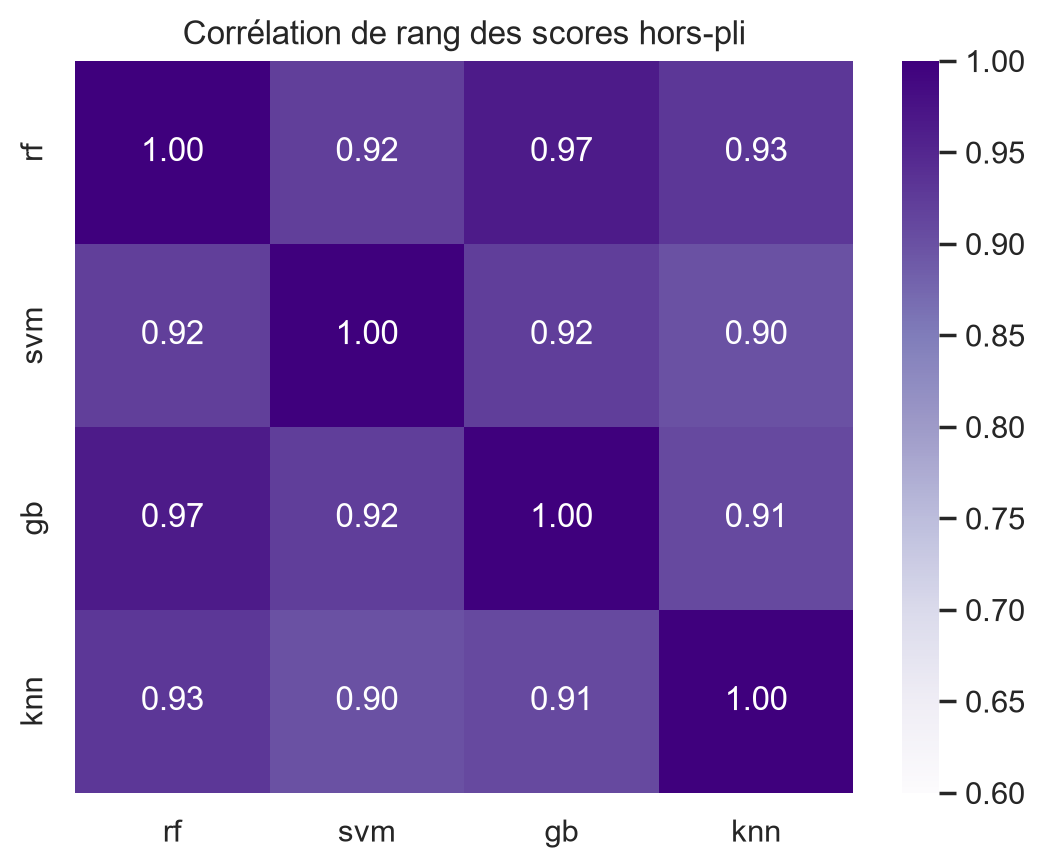
\includegraphics[width=0.5\linewidth]{23_vote_member_correlation.png}
\caption{Corrélation de rang (Spearman) entre les scores hors-pli des quatre membres du vote.}\label{fig:memcorr}
\end{figure}

\begin{figure}[htbp]
\centering
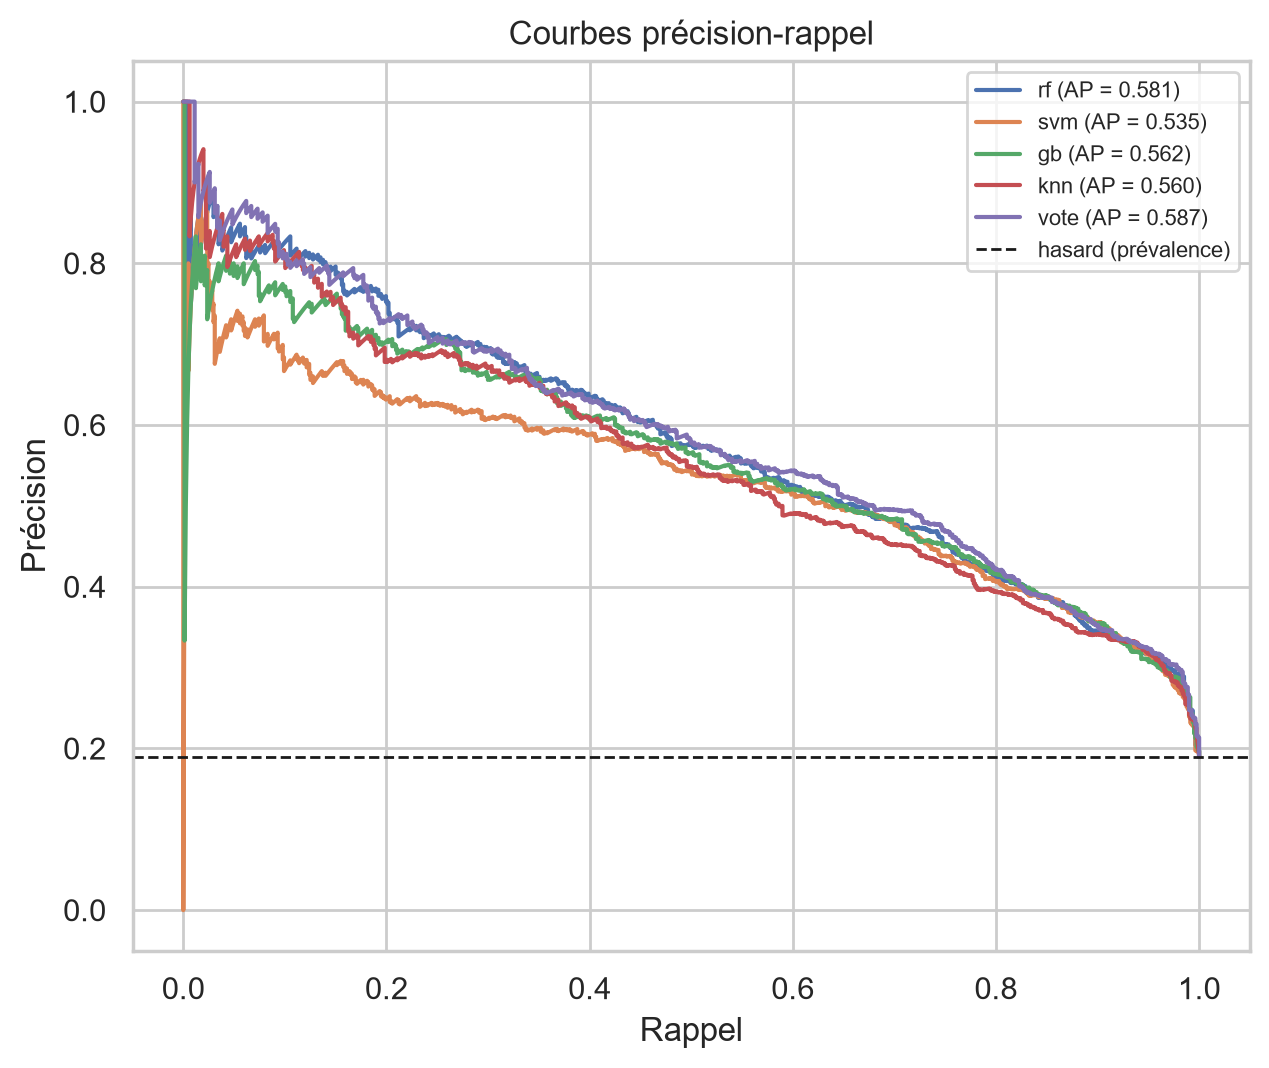
\includegraphics[width=0.75\linewidth]{24_pr_curves_vote.png}
\caption{Courbes précision-rappel hors-pli : membres du vote et vote souple.}\label{fig:prvote}
\end{figure}

\subsection{Évaluation sur le jeu de test}

Le jeu de test ($1\,064$ vins, environ $200$ bons vins) est utilisé pour évaluer le modèle retenu, ainsi que, à titre de comparaison, la forêt seule (tableau~\ref{tab:test}, figures~\ref{fig:testconf} et~\ref{fig:testroc}).

\begin{table}[htbp]
\centering\small
\caption{Performance sur le jeu de test.}\label{tab:test}
\begin{tabular}{@{}lccc@{}}
\toprule
 & Vote (seuil 0,34) & Vote (seuil 0,5) & Forêt (seuil 0,46) \\
\midrule
Accuracy             & 0,812 & 0,854 & 0,798 \\
Précision            & 0,503 & 0,654 & 0,480 \\
Rappel               & 0,728 & 0,495 & 0,757 \\
F1-score             & \textbf{0,595} & 0,563 & 0,587 \\
ROC-AUC              & 0,864 & 0,864 & 0,867 \\
Average precision    & 0,618 & 0,618 & 0,628 \\
\bottomrule
\end{tabular}
\end{table}

\begin{figure}[htbp]
\centering
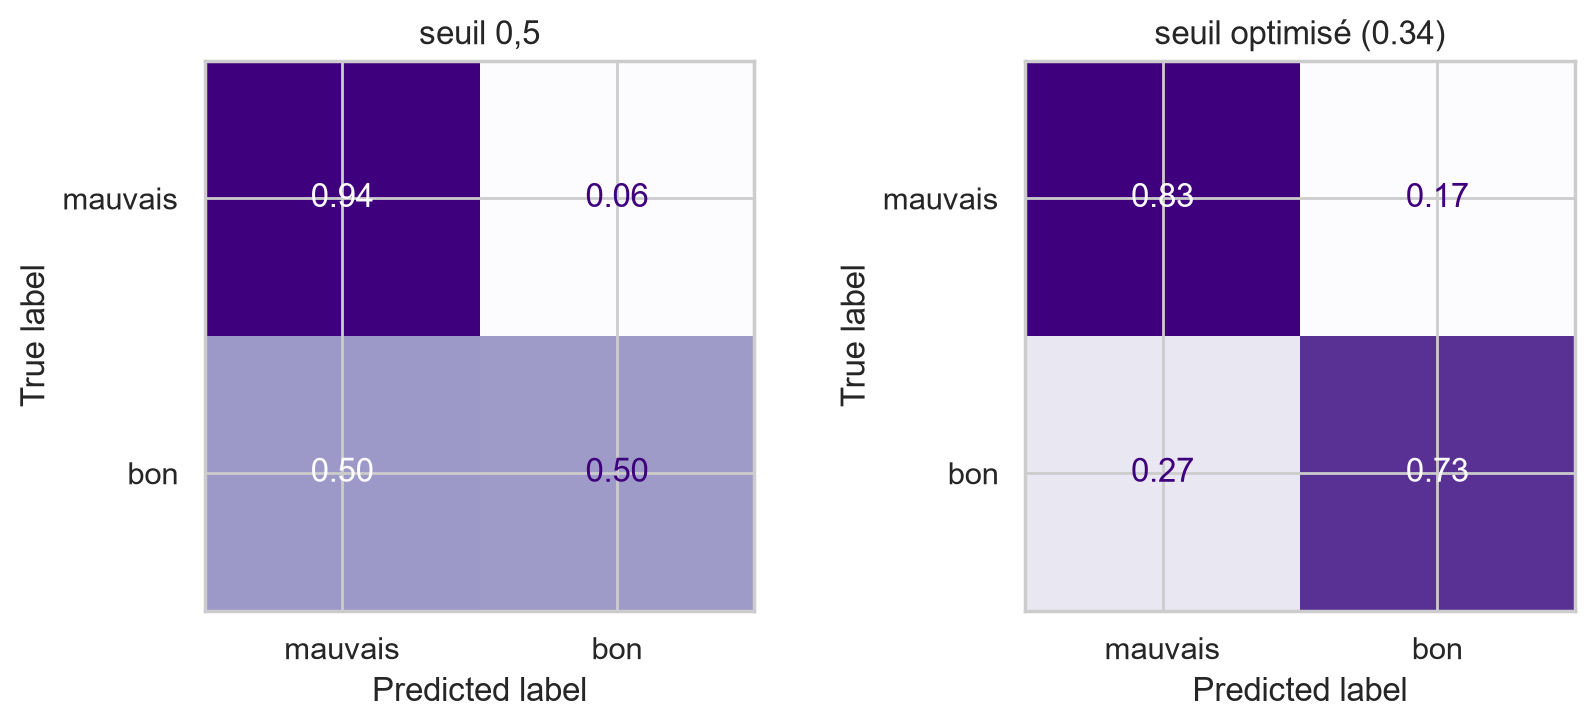
\includegraphics[width=0.9\linewidth]{18_test_confusion.png}
\caption{Matrices de confusion du vote sur le jeu de test (normalisées par ligne), au seuil $0{,}5$ et au seuil optimisé.}\label{fig:testconf}
\end{figure}

\begin{figure}[htbp]
\centering
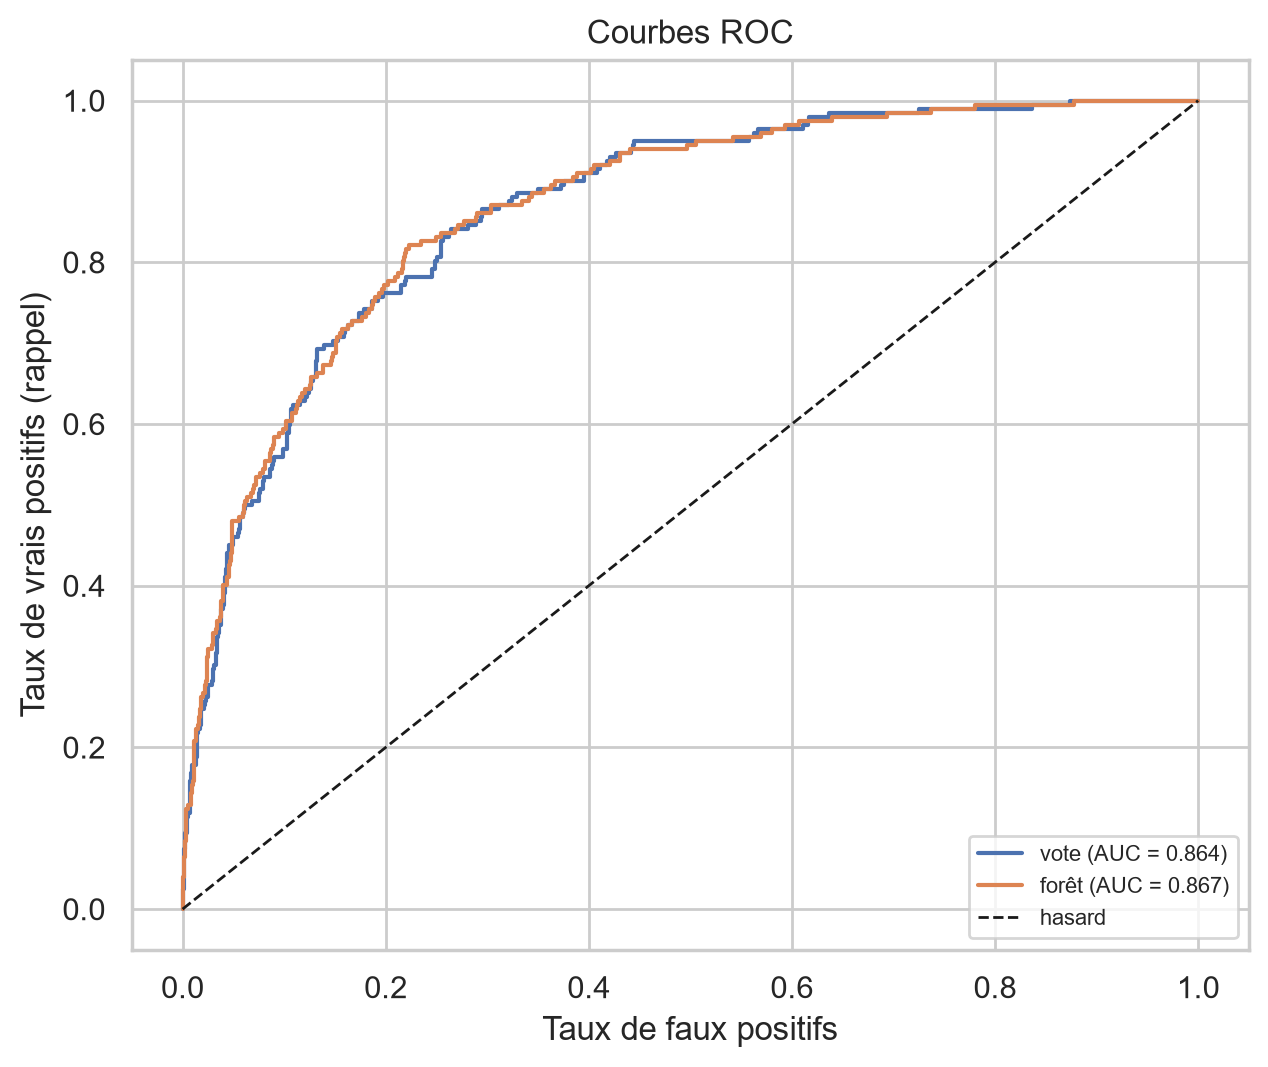
\includegraphics[width=0.7\linewidth]{19_test_roc.png}
\caption{Courbes ROC sur le jeu de test.}\label{fig:testroc}
\end{figure}

\paragraph{Lecture.}
Les résultats de test sont cohérents avec ceux de la validation croisée (AUC $0{,}864$ contre $0{,}859$, F1 $0{,}595$ contre $0{,}585$) : le protocole n'a pas conduit à un sur-ajustement du jeu d'entraînement.
Le seuil optimisé en validation croisée se transfère bien : au seuil $0{,}5$, le F1 tomberait à $0{,}563$ (rappel $0{,}495$, précision $0{,}654$). Le vote détecte $73\,\%$ des bons vins, et environ un vin signalé « bon » sur deux l'est réellement,
alors que la prévalence est de $19\,\%$ : le gain sur le hasard est net mais la qualité reste difficile à prédire à partir des seules mesures chimiques.

\subsection{Incertitude : bootstrap apparié}

Pour comparer le vote à la forêt sans sur-interpréter de petits écarts, nous estimons des intervalles de confiance à 95\,\% par bootstrap apparié (2\,000 rééchantillonnages du jeu de test, mêmes vins pour les deux modèles, seuils fixés ; tableau~\ref{tab:boot}).

\begin{table}[htbp]
\centering\small
\caption{Moyenne bootstrap et intervalle de confiance à 95\,\% sur le jeu de test.}\label{tab:boot}
\begin{tabular}{@{}lccc@{}}
\toprule
 & Vote & Forêt & Différence (vote $-$ forêt) \\
\midrule
ROC-AUC & 0,864 [0,839 ; 0,891] & 0,867 [0,841 ; 0,893] & $-0{,}002$ [$-0{,}008$ ; $+0{,}003$] \\
F1      & 0,595 [0,543 ; 0,643] & 0,587 [0,537 ; 0,636] & $+0{,}008$ [$-0{,}015$ ; $+0{,}030$] \\
\bottomrule
\end{tabular}
\end{table}

Les intervalles de la différence contiennent 0 pour les deux indicateurs : \textbf{sur le test, le vote et la forêt ne sont pas statistiquement distinguables}. Le vote est un peu meilleur en F1 et un peu moins bon en AUC et en AP, sans que l'écart soit significatif.
Il est retenu par la règle définie avant le test, pour sa \textbf{stabilité} : il moyenne quatre modèles et dépend moins d'un réglage unique, ce qui est un argument de robustesse plutôt que de performance.

\subsection{Importance des variables}

L'importance par permutation (baisse du ROC-AUC lorsqu'on permute aléatoirement une colonne du jeu de test, 15 répétitions) est présentée en figure~\ref{fig:perm}. \texttt{alcohol} domine nettement
(perte de $0{,}124$ d'AUC), loin devant les autres variables qui se situent entre $0{,}014$ et $0{,}020$ (SO$_2$ libre, pH, sucre résiduel, sulfates, densité, acidité volatile, chlorures, SO$_2$ total, acide citrique), tandis que
l'acidité fixe ($0{,}005$) et le type ($0{,}001$) sont négligeables. Ce résultat confirme l'analyse exploratoire : l'alcool est le principal discriminant. La densité apparaît moins importante qu'en analyse exploratoire
car elle partage son information avec l'alcool et le sucre résiduel : la permutation répartit l'importance entre variables corrélées.

\begin{figure}[htbp]
\centering
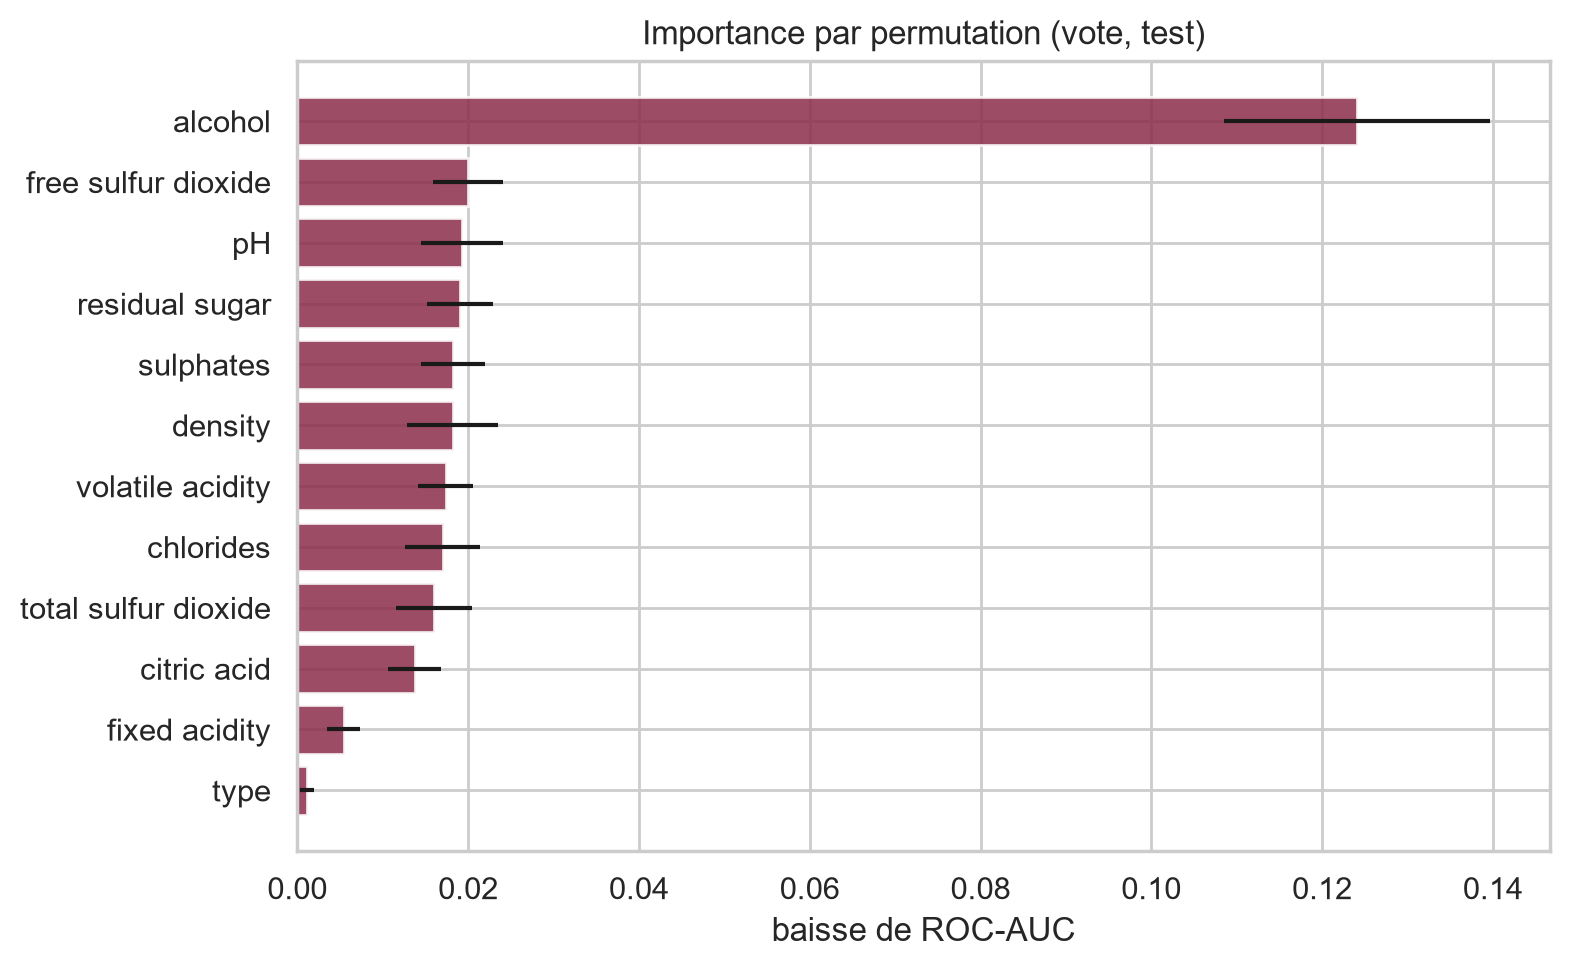
\includegraphics[width=0.75\linewidth]{20_permutation_importance.png}
\caption{Importance par permutation (vote, jeu de test).}\label{fig:perm}
\end{figure}

%% ------------------------------------------------------------------
\section{Mise en œuvre, reproductibilité et application}\label{sec:impl}

\paragraph{Organisation du code.}
Le code réutilisable est regroupé dans le paquet \texttt{src/} : configuration, chargement et découpage des données (\texttt{data.py}), prétraitement et sélection de variables (\texttt{features.py}),
modèles (\texttt{models.py}), évaluation et graphiques (\texttt{evaluate.py}), recherche d'hyperparamètres (\texttt{tuning.py}), vote souple (\texttt{ensemble.py}) et entraînement final (\texttt{train.py}).
Trois notebooks documentent la démarche : exploration, modélisation, optimisation.

\paragraph{Tests unitaires.}
Une suite de 60 tests \texttt{pytest} vérifie le chargement et la fusion des données, le découpage stratifié, l'absence de fuite dans la standardisation, le filtre VIF, chaque sélecteur, chaque modèle,
les métriques (valeurs calculées à la main), les recherches d'hyperparamètres, le vote souple et l'API.

\paragraph{Reproductibilité.}
Les versions des bibliothèques sont figées, la graine est fixée, et la commande \texttt{python -m src.train} reconstruit le modèle final avec les mêmes résultats (seuil $0{,}3432$, ROC-AUC de test $0{,}864$).

\paragraph{API et application web.}
Une API FastAPI expose \texttt{POST /predict} (entrées validées par Pydantic : bornes physiques et \texttt{type} restreint à rouge/blanc) et \texttt{GET /health}. Une page web permet de saisir les mesures d'un vin
et d'obtenir la prédiction, la probabilité et le seuil de décision. Un \texttt{Dockerfile} reconstruit le modèle dans l'image et lance le service sous un utilisateur non privilégié.

%% ------------------------------------------------------------------
\section{Limites et conclusion}

\paragraph{Limites.}
\begin{itemize}
  \item La \textbf{précision reste d'environ $0{,}50$} : un vin signalé bon sur deux ne l'est pas. Le seuil permet d'arbitrer entre précision et rappel selon le coût d'un bon vin manqué ou d'une fausse alerte.
  \item Les \textbf{labels sont subjectifs} (médiane de notes d'experts) et les mesures physico-chimiques n'expliquent qu'une partie du jugement : le plafond ($\text{AUC} \approx 0{,}86$) est partagé par tous les modèles étudiés.
  \item La \textbf{diversité entre les membres du vote est limitée} (corrélations de rang de $0{,}90$ à $0{,}97$), ce qui borne le gain de l'ensemble.
  \item Les estimations issues de la recherche d'hyperparamètres sont légèrement optimistes (le meilleur candidat est choisi sur les mêmes plis) ; seule l'évaluation sur le jeu de test est non biaisée,
        avec une incertitude de l'ordre de $\pm 0{,}03$ sur l'AUC pour environ 200 positifs.
  \item Le modèle est entraîné sur des vins « Vinho Verde » : il ne se généralise pas à d'autres régions ou à d'autres millésimes sans vérification.
\end{itemize}

\paragraph{Conclusion.}
Nous avons construit une chaîne complète de classification de la qualité du vin, sans fuite de données : suppression des doublons, standardisation et sélection à l'intérieur des plis, optimisation par Grid et Random Search,
réglage du seuil sur prédictions hors-pli et évaluation unique sur un jeu de test. Les modèles non linéaires (forêt, SVM, boosting, $k$-NN) dépassent les modèles linéaires ou probabilistes ($\text{AUC} \approx 0{,}85$ contre $0{,}78$--$0{,}83$),
ce qui est cohérent avec la structure non linéaire et bruitée des données. Le modèle final, un vote souple de quatre modèles optimisés, atteint un ROC-AUC de $0{,}864$ et un F1 de $0{,}595$ sur le test, à un niveau
statistiquement équivalent à celui de la meilleure forêt. L'\textbf{alcool} est le principal déterminant de la qualité, très loin devant les autres variables. Le principal levier d'amélioration n'est plus algorithmique mais lié à l'information disponible :
variables supplémentaires (cépage, millésime, notes de dégustation détaillées) ou modèle exploitant la note ordinale (0 à 10) plutôt que la seule cible binaire.

\begin{thebibliography}{9}
\bibitem{cortez2009} P.~Cortez, A.~Cerdeira, F.~Almeida, T.~Matos et J.~Reis. \emph{Modeling wine preferences by data mining from physicochemical properties}. Decision Support Systems, 47(4):547--553, 2009.
\bibitem{sklearn} F.~Pedregosa et al. \emph{Scikit-learn: Machine learning in Python}. Journal of Machine Learning Research, 12:2825--2830, 2011.
\bibitem{breiman2001} L.~Breiman. \emph{Random forests}. Machine Learning, 45(1):5--32, 2001.
\bibitem{bergstra2012} J.~Bergstra et Y.~Bengio. \emph{Random search for hyper-parameter optimization}. Journal of Machine Learning Research, 13:281--305, 2012.
\bibitem{platt1999} J.~Platt. \emph{Probabilistic outputs for support vector machines and comparisons to regularized likelihood methods}. Dans \emph{Advances in Large Margin Classifiers}, MIT Press, 61--74, 1999.
\end{thebibliography}

\end{document}
